\documentclass[12pt,a4paper,twoside]{report}

\usepackage[utf8]{inputenc}
\usepackage{graphicx}
\graphicspath{ {./../figures/} }
\usepackage{caption}
\usepackage{subcaption}
\usepackage{xcolor}
\usepackage{fancyvrb} % Verbatim and coloring therein
\usepackage{hyperref}
\usepackage{imakeidx} % for index
\makeindex[columns=3, title=Alphabetical Index]
\usepackage{soul} % allow wrapping of underlined text, via \ul{...}
\usepackage{natbib} % for bibliography
\usepackage[left=2cm,right=2cm]{geometry} % somewhat wider text to allow code
\usepackage{siunitx} %% SI Units
\usepackage{amsmath,bm} %% for math ...
\usepackage{amssymb} %% greek and various toher characters and symbols ...
\usepackage{mathabx}
\usepackage[acronym, toc, nonumberlist]{glossaries} %% for acronyms
\usepackage{tabularx}
\usepackage{multirow} %% for tabular

%% TikZ stuff %%
\usepackage{tikz} % add a few drawings ...
\usepackage{tkz-euclide}
\usetikzlibrary{matrix}
\usetikzlibrary{shapes.geometric, arrows} % for creating tikz flowcharts 
\usetikzlibrary{shapes.misc}
\usetikzlibrary{calc}
\usetikzlibrary{quotes,angles}
\tikzstyle{io} = [trapezium, trapezium left angle=70, trapezium right angle=110, minimum width=3cm, minimum height=1cm, text centered, draw=black, fill=blue!30]
\tikzstyle{process} = [rectangle, minimum width=3cm, minimum height=1cm, text centered, draw=black, fill=orange!30]
\tikzstyle{decision} = [diamond, minimum width=3cm, minimum height=1cm, text centered, draw=black, fill=green!30]
\tikzstyle{arrow} = [thick,->,>=stealth]

\usepackage{listings} % include source code files
% Solarized colour scheme for listings
\definecolor{solarized@base03}{HTML}{002B36}
\definecolor{solarized@base02}{HTML}{073642}
\definecolor{solarized@base01}{HTML}{586e75}
\definecolor{solarized@base00}{HTML}{657b83}
\definecolor{solarized@base0}{HTML}{839496}
\definecolor{solarized@base1}{HTML}{93a1a1}
\definecolor{solarized@base2}{HTML}{EEE8D5}
\definecolor{solarized@base3}{HTML}{FDF6E3}
\definecolor{solarized@yellow}{HTML}{B58900}
\definecolor{solarized@orange}{HTML}{CB4B16}
\definecolor{solarized@red}{HTML}{DC322F}
\definecolor{solarized@magenta}{HTML}{D33682}
\definecolor{solarized@violet}{HTML}{6C71C4}
\definecolor{solarized@blue}{HTML}{268BD2}
\definecolor{solarized@cyan}{HTML}{2AA198}
\definecolor{solarized@green}{HTML}{859900}

% Define C++ syntax highlighting colour scheme
\lstset{language=C++,
        basicstyle=\footnotesize\ttfamily,
        numbers=left,
        numberstyle=\tiny,
        tabsize=2,
        breaklines=true,
        escapeinside={@}{@},
        numberstyle=\tiny\color{solarized@base01},
        keywordstyle=\color{solarized@green},
        stringstyle=\color{solarized@cyan}\ttfamily,
        identifierstyle=\color{solarized@blue},
        commentstyle=\color{solarized@base01},
        emphstyle=\color{solarized@red},
        frame=single,
        rulecolor=\color{solarized@base2},
        rulesepcolor=\color{solarized@base2},
        showstringspaces=false
}

% include the external source file, instead of pasting its contents directly 
% into the LaTeX documen
\newcommand{\codelst}[1]{\lstinputlisting[caption=\texttt{\protect\detokenize{#1}}]{#1}\newpage}

% augment the paragraph skip ... a bit more clear text
\setlength{\parskip}{1em}

\bibliographystyle{plainnat}

\makeglossaries
\newacronym{ids}{IDS}{International DORIS Service}
\newacronym{antex}{ANTEX}{Antenna Exchange Format}
\newacronym{pcv}{PCV}{Phase Center Variations}
\newacronym{pco}{PCO}{Phase Center Offset}
\newacronym{iers}{IERS}{International Earth Rotation and Reference Systems Service}
\newacronym{era}{ERA}{Earth Rotation Angle}
\newacronym{tio}{TIO}{Terrestrial Intermediate Origin}
\newacronym{cio}{CIO}{Celestial Intermediate Origin}
\newacronym{cip}{CIP}{Celestial Intermediate Pole}
\newacronym{vlbi}{VLBI}{Very Long Baseline Interferometry}
\newacronym{ode}{ODE}{Ordinary Differential Equation}
\newacronym{rkn}{RKN}{Runge-Kutta-Nystr{\"o}m}
%\newacronym{}{}{}

\title{PhD Memo and Notes}
\author{Xanthos}
\date{\today}

\begin{document}

\begin{titlepage}
\maketitle
\end{titlepage}

%\frontmatter
\tableofcontents
\listoffigures
\listoftables

\section{\gls{doris} Observation Equation}\label{sec:doris-observation-equation}

\begin{figure}
  \centering
  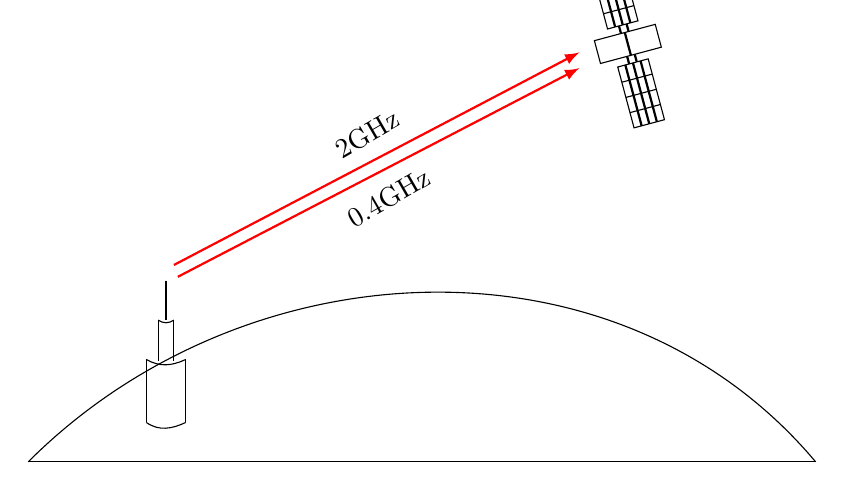
\begin{tikzpicture}
    \coordinate (lend) at (-5, 0);
    \coordinate (rend) at (5, 0);
    \draw (lend) to (rend);
    \draw (lend) to[out=45,in=-230] (rend);

    \coordinate (blb) at (-3.5, 0.5);
    \coordinate (brb) at (-3, 0.5);
    \draw (blb) to[out=-35,in=205] (brb);

    \coordinate (mlb) at (-3.5, 1.3);
    \coordinate (mrb) at (-3, 1.3);
    \draw (mlb) to[out=-30,in=205] (mrb);
    %\draw (mlb) to[out=35,in=-205] (mrb);
    \draw (blb) to (mlb);
    \draw (brb) to (mrb);
    
    \coordinate (tlb) at (-3.35, 1.8);
    \coordinate (trb) at (-3.15, 1.8);
    \draw (tlb) to[out=-35,in=215] (trb);
    \draw (tlb) to (-3.35, 1.28);
    \draw (trb) to (-3.15, 1.28);

    \coordinate (ulb) at (-3.26, 2.3);
    \coordinate (urb) at (-3.24, 2.3);
    \draw (ulb) to (-3.26, 1.8);
    \draw (urb) to (-3.24, 1.8);

    \rotatebox{15}{%
    \draw[] (3.5,4.6) rectangle (4.3,4.3);
    % Up panel
    \draw[thick] (3.9,4.3) to (3.9,4.6);
    \draw[thick] (3.85,4.6) to (3.85,4.7);
    \draw[thick] (3.95,4.6) to (3.95,4.7);
    \draw[] (3.7,5.5) rectangle (4.1,4.7);
    % grid
    \draw[thick] (3.8,4.7) to (3.8, 5.5); 
    \draw[thick] (3.9,4.7) to (3.9, 5.5); 
    \draw[thick] (4.0,4.7) to (4.0, 5.5); 
    \draw[] (3.7,4.9) to (4.1, 4.9);
    \draw[] (3.7,5.1) to (4.1, 5.1);
    \draw[] (3.7,5.3) to (4.1, 5.3);
    % Down panel
    \draw[thick] (3.85,4.3) to (3.85,4.2);
    \draw[thick] (3.95,4.3) to (3.95,4.2);
    \draw[] (3.7,3.4) rectangle (4.1,4.2);
    % grid
    \draw[thick] (3.8,3.4) to (3.8, 4.2); 
    \draw[thick] (3.9,3.4) to (3.9, 4.2); 
    \draw[thick] (4.0,3.4) to (4.0, 4.2); 
    \draw[] (3.7,3.6) to (4.1, 3.6);
    \draw[] (3.7,3.8) to (4.1, 3.8);
    \draw[] (3.7,4.0) to (4.1, 4.0);
    }
    
    \coordinate (satant1) at (2.0,  5.2);
    \coordinate (bcnant1) at (-3.15,2.5);
    \coordinate (satant2) at (2.0,  5.0);
    \coordinate (bcnant2) at (-3.10,2.35);
    \draw[thick,red,-latex] (bcnant1) -- node[above=1mm, align=center, black, rotate=30]{2GHz} (satant1);
    \draw[thick,red,-latex] (bcnant2) -- node[below=1mm, align=center, black, rotate=30]{0.4GHz} (satant2);

\end{tikzpicture}

  \caption{\gls{doris} System Description}
  \label{fig:doris-system-description}
\end{figure}

\subsection{Theoretical Model of Doppler Observations}\label{ssec:doris-obs-theory}
A detailed derivation of the Doppler observation equation, as implemented via the 
\gls{doris} system, can be found in \cite{Lemoine2016}, including a thorough theoretical 
discussion. A brief overview is only given here, with focus on model implementation.

To gain a clear view on the model of the measurements, a rigorous disctinction of 
events must be made; four different events can be identified:
\begin{description}
    \item[beginning of emission] of the 1\textsubscript{st} cycle by the emitter, 
    \(\tau_{e_1}\) in the proper time scale of the emitter and \(t_1\) in the coordinate 
    time
    
    \item[beginning of reception] of the the 1\textsubscript{st} cycle by the receiver, 
    \(\tau_{r_1'}\) in the proper time scale of the receiver and 
    \(t_{1'}\) in the coordinate time

    \item[end of emission] of the N\textsubscript{th} cycle by the emitter, 
    \(\tau_{e_2}\) in the proper time scale of the emitter and \(t_2\) in the coordinate 
    time
    
    \item[end of reception] of the N\textsubscript{th} cycle by the receiver, 
    \(\tau_{r_2'}\) in the proper time scale of the receiver and 
    \(t_{2'}\) in the coordinate time
\end{description}

During the proper time interval $\Delta\tau_{r} = \tau_{r2'} - \tau_{r1'}$, 
the receiver has received the $N_e$ cycles sent by the emitter, with $N_e = f_e \Delta\tau_e$, 
$f_e$ being the proper frequency of the emitter. The receiver is also equipped with
an oscilator and during the proper time interval $\Delta\tau_{r}$ has generated 
a number $N_r = f_r \Delta\tau_r$ of cycles, $f_r$ being the proper frequency of the 
receiver.

The Doppler measurement is the count, by the receiver electronics, of the number 
of cycles of difference between \(N_e\) and \(N_r\):
\begin{equation}
    \begin{split}
    N_{DOP} & = N_e - N_r\\
            & = f_e \Delta\tau_e - f_r \Delta\tau_r
    \end{split}
\end{equation}

\emph{In the RINEX files, this Doppler count is the difference between two phase measurements 
done at different time tags in the proper time-scale of the receiver.}

After a series of assumptions and simplifications, theoretical formula for the 
Doppler count can be written as (\cite{Lemoine2016}):
\begin{equation}
    \begin{split}
        \frac{c}{f_e \Delta\tau_r} N_{DOP} & \approx c \frac{f_e - f_r}{f_e} \\
        & - (1 - \frac{U_e}{c^2} - \frac{{V_e}^2}{2 c^2}) \frac{\rho_2 - \rho_1}{\Delta\tau_r}\\
        & + \frac{1}{c} (U_r - U_e + \frac{{V_r}^2 - {V_e}^2}{2}) \\
        & + \frac{2 \mu}{c^2 \Delta\tau_r} [\ln{(\frac{R_1 + R_{1'} + \rho_1}{R_1 + R_{1'} - \rho_1})} - \ln{(\frac{R_2 + R_{2'} + \rho_2}{R_2 + R_{2'} - \rho_2})}]
    \end{split}
\end{equation}
where
\begin{description}
  \item $c$ is the velocity of light in vacuum,
  \item $f_e$ and $f_r$ are the emitter's and receiver's proper frequencies,
  \item $U_e$ and $U_r$ are the gravitational potential at the emitter and receiver,
  \item $V_e$ and $V_r$ is the velocity of the clock at the emitter and receiver 
    (in the coordinate reference frame),
  \item $\rho _i$ is the curvlinear trajectory (of the photon(s)) at the event $i$,
  \item $R_i$ is the geometric distance between the beacon and the satellite at event $i$
\end{description}

The above equation can be conviniently split into two parts, one containing the ``measured'' 
quantities and one with the ``theoretical'' terms, as 
\begin{subequations}\label{eq:lem12}
  \begin{align}
    v_{measured} & = \frac{c}{f_e} (f_e - f_r -
     \frac{N_{DOP}}{\Delta\tau_r}) + \Delta u_{REL} \label{eq:lem12a} \\
    v_{theo}     &= \frac{\rho_2 - \rho_1}{\Delta\tau_r} (1- \frac{U_e}{c^2} - 
      \frac{{V_e}^2}{2 c^2}) \label{eq:lem12b}
  \end{align}
\end{subequations}
with
\begin{equation}
    \begin{split}
        \Delta v_{REL} &= \frac{1}{c} (U_r - U_e + \frac{{V_r}^2 - {V_e}^2}{2}) \\
        & + \frac{2 \mu}{c^2 \Delta\tau_r} [\ln{(\frac{R_1 + R_{1'} + \rho_1}{R_1 + R_{1'} - \rho_1})} - \ln{(\frac{R_2 + R_{2'} + \rho_2}{R_2 + R_{2'} - \rho_2})}]
    \end{split}
\end{equation}

It is well known that signals transmitted through the Earth's atmosphere are affected by 
it (delayed); let $\Delta v_{IONO}$ and $\Delta v_{TROPO}$, be the propagation corrections of 
the radio electric signal through the ionosphere and troposphere respectively. 

Additionaly, in the actual case (measurements), the nominal frequencies $f_e$ and $f_r$ 
are not the ``true'' ones; hence a relative correction needs to be applied (e.g. for the 
emmiter) $f_{e_T} = f_{e_N} (1 + \frac{\Delta f_e}{f_{e_N}})$, where the subscript $T$ 
denotes the ``True'' frequency and $N$ the nominal one. Thus in \autoref{eq:lem12} the 
terms $f_e$ and $f_r$ need to be substituted by $f_{e_T}$ and $f_{r_T}$ respectively.

$\Delta v_{IONO}$ and $\Delta v_{REL}$, which do not involve adjusted parameters, can be placed 
on the ``measured'' part of \autoref{eq:lem12} and $\Delta v_{TROPO}$ and $\frac{\Delta f_e}{f_{e_N}}$ 
on the ``theoretical'' part. Furthermore, since $\Delta f_e / f_{e_N} \ll 1$ all in 
including $\Delta f_e / f^2_{e_N}$ and $\Delta f^2_e / f^2_{e_N}$ can be safely neglected and 
\autoref{eq:lem12} can be written as:
\begin{subequations}\label{eq:lem13}
    \begin{align}
        v_{measured} & = \frac{c}{f_{e_N}} (f_{e_N} - f_{r_T} -
          \frac{N_{DOP}}{\Delta\tau_r}) + \Delta u_{REL} + 
          \Delta u_{IONO} \label{eq:lem13a} \\
        v_{theo} &= \frac{\rho_2 - \rho_1}{\Delta\tau_r} 
          (1- \frac{U_e}{c^2} - \frac{{V_e}^2}{2 c^2}) + 
          \Delta u_{TROPO} - \frac{c(\frac{N_{DOP}}{\Delta\tau_r} + 
          f_{r_T})}{f_{e_N}} \frac{\Delta f_e}{f_{e_N}} \label{eq:lem13b}
    \end{align}
\end{subequations}
where 
\begin{description}
    \item[\(v_{measured}\)] is the measured relative velocity between the emitter and 
    the receiver between the events 1' and 2', based on the Doppler count \(N_{DOP}\), 
    corrected for the ionospheric and relativistic effects.

    \item[\(v_{theo}\)] is the the theoretical (computed) emitter/receiver relative velocity 
    between the events 1' and 2', corrected for the tropospheric effect and for a solved-for 
    frequency bias \(\frac{\Delta f_e}{f_{e_N}}\) of the emitter. 
    \(f_{r_T} = f_{r_N} (1 + \frac{\Delta f_r}{f_{r_N}})\) 
    is an estimate of the proper frequency of the receiver.

    \item[\(\Delta v_{REL} = \Delta v_{{REL}_c} + \Delta v_{{REL}_r}\)] is the relativistic 
    correction, composed of two parts: the clock correction \(\Delta v_{{REL}_c}\) and the 
    travel correction \(\Delta v_{{REL}_r}\)
    \begin{subequations}\label{eq:lem14}
        \begin{align}
            \Delta v_{{REL}_c} & = \frac{1}{c} 
              (U_r - U_e + \frac{{V_r}^2 - {V_e}^2}{2}) \label{eq:lem14a}\\
            \Delta v_{{REL}_r} & = \frac{2 \mu}{c^2 \Delta\tau_r} \left[ 
              \ln{(\frac{R_1 + R_{1'} + \rho_1}{R_1 + R_{1'} - \rho_1})} - 
              \ln{(\frac{R_2 + R_{2'} + \rho_2}{R_2 + R_{2'} - \rho_2})} \right] \label{eq:lem14b}
        \end{align}
    \end{subequations}
\end{description}

Note that \autoref{eq:lem13} can be further simplified to \autoref{eq:lem17} by 
ommiting small terms (\autoref{ssec:small-terms}).

%\emph{Usually, one frequency offset and one tropospheric zenithal bias are adjusted per pass.}

\subsection{Implementation of the Doppler Observation Model}\label{ssec:obs-model-implementation}

\subsubsection{Small Terms}\label{sssec:small-terms}
In \autoref{eq:lem13}, the smallest terms are \(-U_e / c^2 - {V_e}^2 / 2 c^2\) and 
\(\Delta v_{{REL}_T}\); in the case of \gls{doris} they ammount to \num{11.} and 
\num{6.} \SI{10e-6}{\meter\per\second} respectively (\cite{Lemoine2016}). 
Furthermore, since the emitters are located on the ground, the term 
\(-U_e / c^2 - {V_e}^2 / 2 c^2\) is constant per station. This small 
relativistic offset is absorbed by the adjustment of \(\Delta f_e / f_{e_N}\). 
So it is possibly to furher simplify \autoref{eq:lem13} to:
\begin{subequations}\label{eq:lem17}
    \begin{align}
        v_{measured} & = \frac{c}{f_{e_N}} (f_{e_N} - f_{r_T} -
          \frac{N_{DOP}}{\Delta\tau_r}) + 
          \Delta u_{{REL}_C} + \Delta u_{IONO} \label{eq:lem17a}\\
        v_{theo} &= \frac{\rho_2 - \rho_1}{\Delta\tau_r} + \Delta u_{TROPO} - 
          \frac{c(\frac{N_{DOP}}{\Delta\tau_r} + f_{r_T})}{f_{e_N}} 
          \frac{\Delta f_e}{f_{e_N}} \label{eq:lem17b}
    \end{align}
\end{subequations}

\subsubsection{Correction of Aberration}\label{sssec:doris-aberration}
In \autoref{eq:lem13} (or \autoref{eq:lem17}), $\rho _i$ is the geometrical distance 
between the emitter at time $t_i$ and the receiver at time $t_{i'}$ (with $i=1,2$). 
The measurements are made by the receiver electronics, hence the instance $t_i$ is 
actually unknown. In order to compute accurately $t_i$ and thus the position of 
the emitter at this istant in time, a \emph{correction of aberration} (\cite{Lemoine2016}) 
has to be performed. This correction can be evaluated in an iterative manner: an 
approximate value of of the emitter-receiver distance $\rho ^{*} _i$ is first computed, 
by evaluating the position of the beacon at time $t_{i'}$. Subsequently, $t_i$ can be 
found via $t_i = t_{i'} - \rho ^{*} _i / c$. In practice, one iteration is enough.

\subsubsection{Geopotential}\label{sssec:doris-geopotential}
For a station on the geoid, the potential at the level of the station is the sum 
of the gravitational potential and the centrifugal potential due to the Earth's 
rotation: $U_{GEO} = U_e + \frac{{V_e}^2}{2}$, which is a constant. For a station 
not located on the geoid, the quantity $U_e + \frac{{V_e}^2}{2}$ will only depend 
on the height of the beacon above the geoid.

For the computation of the gravitational potential for \gls{leo} satellites, 
the pottential $U_r$ cannot be restricted to the central term only ($GM_{\Earth} / r$) and
the Earth's oblateness ($J_2$) effect should also be considered (\cite{Larson2007}). 
Hece, the equation used reads (\cite{Lemoine2016})
\begin{equation}\label{eq:lem18}
  U_r = 
    -\frac{GM_{\Earth}}{r} \left( 
      1 - 
      \left( \frac{R_{\Earth}}{r} \right) ^2 
      J_2 \frac{3 sin^2(\phi) - 1}{2} 
    \right)
\end{equation}
or in cartesian coordiates (\cite{Larson2007})
\begin{equation}
  U_r = -\frac{GM_{\Earth}}{r} \left( 1- \left(\frac{R_{\Earth}}{r}\right)^2 
    J_2 \frac{3 z^2 - r^2}{2r^2} \right)
\end{equation}
with $R_{\Earth}$ the equatorial radious of the earth, $r$ radial 
distance of the satellite (to the Earth's center), $\phi$ latitude of the 
satellite and $J_2 = 1.0826359 \dot 10^{-3}$ in the zero-tide system (\cite{iers2010}).

\subsubsection{True Proper Frequency of the Receiver}\label{sssec:true-proprtfrequency-of-the-receiver}
For the term $f_{r_T}$ that appears in \autoref{eq:lem13}, we need an estimate of 
$\Delta f_{r} / f_{r_N}$. This estimate can be obtained in one of the following ways 
\cite{Lemoine2016}:
\begin{enumerate}
    \item via the field ``F'' recorded for every single measurement in the \gls{doris} 
      RINEX file (see \autoref{ssec:relative-frequency-offset}); not that this estimation 
      is not very smooth, as noticed by \cite{Gao2015} and it is advisable, before 
      using it in \autoref{eq:lem13}, to perform a linear (or polynomial) regression of 
      these estimates over one or a few days.
    \item It can also be obtained from a polynomial regression
      over the frequency offsets estimated during the passes
      over the master beacons
    \item It can finally be estimated by the users themselves as a
      by-product of their re-computation of the timetagging polynomial (see \cite{Mercier2010})
\end{enumerate}

\subsubsection{Nominal Receiver \& Emitter Frequencies}\label{ssec:nominal-frequencies}
In the observation equation model \autoref{eq:lem13} we distinguish between 
\emph{nominal} and \emph{true} receiver/emitter frequencies, to account for 
the fact that in ``real world'' these two are not actually equal.

\paragraph{Emitter (Beacon) Nominal Frequencies, $f_{e_N}$}\label{par:beacon-nominal-frequencies}
RINEX file headers, contain values of the \emph{station frequency shift 
factor} $k$ for each of the beacons involved (\cite{DORISRNX3}, Sec. 6.16). 
These are used to compute the ``nominal'' frequencies of the beacon/emitter 
(usually, this shift factor is just $0$, but it can be an integer 
$k \neq 0$). The frequencies are computed as (\cite{DORISRNX3}, Sec. 6.16):
\begin{equation}
  \begin{aligned}
    L_{2GHz}   &= 543 \cdot F_0 \left( \frac{3}{4} + \frac{87\cdot k}{5 \cdot 2^{26}} \right) \\
    L_{400MHz} &= 107 \cdot F_0 \left( \frac{3}{4} + \frac{87\cdot k}{5 \cdot 2^{26}} \right) 
    \label{eq:nominal-freq}
  \end{aligned}
\end{equation}
where $F_0 = 5e6 \text{ Hz}$ the \gls{uso} frequency. These value, are the ones 
labelled as $f_{e_N}$ in \autoref{eq:lem13}.

The \emph{true proper frequency} of the emitter $f_{e_T}$, can be computed 
from:
\begin{equation}
  f_{e_T} = f_{e_N} \cdot \left( 1 + \frac{\Delta f_e}{f_{e_N}} \right)
\end{equation}
but the quantity $\Delta f_e / f_{e_N}$ is not know a-priori and has to be 
estimated during the processing.

The quantity $\Delta f_e / f_{e_N}$  can be estimated either as a constant term (bias), 
or using a linear model (bias ad drift). In the latter case (followed in this Thesis), 
the model can be written as:
\begin{equation}
  \frac{\Delta f_e}{f_{e_N}}\at{\tau=\tau _i} = \alpha + \beta \cdot \delta \tau
\end{equation}
%with an a-priori value of 0 and no process noise. 
For the estimation, we need the partials of the observation equation \autoref{eq:lem13b} 
w.r.t. the $\alpha$ and $\beta$ parameters, which are:
\begin{equation}
  \begin{aligned}
  \frac{\partial v_{theo}}{\partial \alpha} &= 
    \frac{c(\frac{N_{DOP}}{\Delta\tau_r} + f_{r_T})}{f_{e_N}} \\
  \frac{\partial v_{theo}}{\partial \beta} &= 
    \frac{c(\frac{N_{DOP}}{\Delta\tau_r} + f_{r_T})}{f_{e_N}} \cdot \delta \tau
  \end{aligned}
\end{equation}

\paragraph{Receiver True Proper Frequency $f_{r_T}$}\label{par:receiver-true-proper-frequency}
In \autoref{eq:lem13}, $f_{r_T}$ is the \emph{true proper frequency of 
the receiver} with nominal value 
\begin{equation}\label{eq:frt-gen}
  f_{r_T} = f_{r_N} \cdot \left( 1 + \frac{\Delta f_r}{f_{r_N}} \right)
\end{equation}
where $f_{r_N}$ is the ``nominal'' frequency value.

In practice the value $\Delta f_r / f_{r_N}$, called the \emph{relative 
frequency offset} of the receiver, is given in the RINEX files for each epoch 
(under the observable tagged \texttt{F}). Note that these values are scaled to 
$10^{-11}$ (\cite{DORISRNX3}, Sec. 6.11), so that for a given epoch $t_i$, the 
true frequency is
\begin{equation}\label{eq:frt-rinex}
  f_{r_T}\at{t=t_i} = f_{r_N} \cdot \left( 1 + F_{t_i} \cdot 10^{-11} \right)
\end{equation}
where $F_{t_i}$ is the relative frequency offset value recovered from the RINEX 
file.

\iffalse
\fi

\subsection{Ionospheric Correction}\label{ssec:iono-correction}
The basic observation equation \autoref{eq:lem13}, is formed for the \SI{2}{\GHz} 
carrier. For each measurement, the ionospheric path delay has to be corrected for, 
by computing a correction (in cycles) as (\cite{Lemoine2016}, Sec. 2.5.7):
\begin{equation}
  \delta_{ION} [\SI{2}{\GHz}\text{ cycles}] = 
    \frac{L_{\SI{2}{\GHz}} - \sqrt{\gamma} \cdot L_{\SI{400}{\MHz}}}{\gamma - 1}
  \label{eq:iono-delay-cycles}
\end{equation}
which is added to the \SI{2}{\GHz} measurement at time $t=t_i$ (obtained by the 
RINEX file). Thus, the corrected observation is:
\begin{equation}\label{eq:l2if}
  L_{\SI{2}{\GHz},IF} [\SI{2}{\GHz}\text{ cycles}] = 
    L_{\SI{2}{\GHz}} + \delta_{ION}
\end{equation}

Note that after applying \autoref{eq:l2if}, the measurement is refered to the ``Iono-Free'' 
geometrical endpoints of the signal path (and not the \SI{2}{\GHz} endpoints). 
This means that the respective {phase center corrections (i.e. \gls{pco} and \gls{pcv})
both at the satellite and at the beacon have to be applied.

\section{DORIS RINEX}\label{sec:doris-rinex}
With the adoption of the \gls{doris} DGXX receivers, first installed onboard the 
Jason-2 satellite, signal tracking on seven different channels simultaneously became 
possible, with synchronous dual frequency phase and pseudo-range measurements 
(\cite{Mercier2010}). This development made it possible for \gls{doris} data to 
be described in a manner similar to \gls{gnss} data, and hence an extension of the 
RINEX 3.0 format (\cite{RINEX305}) was defined and adopted for \gls{doris} observations to be 
recorded and published in. One major advantage of these new measurement data is 
that they are available with a very short latency (older data needed to be pre-processed 
before published). The new data exchange format is expected to further aid analysis 
development, since it allows each analysis center to be independent from \gls{cnes}
data preprocessing, as users have access to synchronous phase and 
pseudorange measurements (\cite{Cerri2011}).

\subsection{General Format Description}
The \gls{doris} RINEX format consists of one ASCII file containing both space based 
and meteorological data collected at \gls{doris} stations and relayed by satellites.
It bears close resemblance to the GNSS RINEX Version 3 (\cite{RINEX305});
data files consist of a header section and a data section. The first contains 
global information for the entire file, while the latter contains the actual 
observations and a date tag, keeping strict chronological order.
Observation types recorded in the DORIS RINEX files are the given in 
\autoref{table:doris-rinex-observation-types}.

\gls{doris} is basically running on its own proper time which is constantly linked 
to \gls{tai}. Time tags are given in instrument time, and clock offset values are 
provided between instrument time and \gls{tai}.

\begin{table}[h!]
  \centering
  \begin{tabular}{|c c c|}
  \hline
  Descriptor & Observation Type & Units \\
  \hline
  \texttt{L} & carrier phase observation & cycles \\
  \texttt{C} & pseudo-range observation & \si{\metre}\\
  \texttt{W} & power level received at each frequency & \si{\dBm} \\
  \texttt{F} & relative frequency offset of the receiver’s oscillator $\frac{f-f_0}{f_0}$ & $10^{-11}$ \\
  \texttt{P} & ground pressure at the station & 100 \si{\pascal} (\si{\milli\bar}) \\
  \texttt{T} & ground temperature at the station & \si{\degreeCelsius} \\
  \texttt{H} & ground humidity at the station & \si{\percent} \\
  \hline
  \end{tabular}
  \caption{\gls{doris} RINEX observation types.}
  \label{table:doris-rinex-observation-types}
\end{table}
A detailed description of the data files, can be found in \cite{DORISRNX3}.

\iffalse
\subsection{Receiver Clock Offsets}
DORIS RINEX contain a ``receiver clock offset'' \(\tau_{r_{offset}}\) (as an 
optional field) at the header record of every epoch. E.g. the line
\begin{verbatim}
    ...
    > 2020 01 01 00 00 35.099949800  0  1       -3.248177132 0
    ...
\end{verbatim}
records a receiver clock offset of \SI{35.099949800}{\second} followed by the 
receiver clock offset flag, which in this case is \num{0}. In such record 
lines, the date (given as YYYY MM DD HH MM SS.) is given in the on-board time 
scale (aka proper time of the receiver) and the conversion to the \gls{tai} 
time scale is obtained by adding the receiver clock offset.

\textit{Depending on the version of the RINEX file, this offset can have been either 
computed by the DORIS-DIODE navigator, or through a post-fit processing using PANDOR. 
In the first case, the file ends with ``.001'' whereas in the second with ``.010''. 
More information on the computation of (\(\tau_{r_{offset}}\) are provided in 
\cite{lemoine-2016}.}

\subsection{Types of DORIS measurements}\label{ssec:types-of-doris-measurements}

\subsubsection{Relative Frequency Offset}\label{sssec:relative-frequency-offset}
\gls{doris} RINEX files (usually) contain a measurement type labeled ``F'' (should be 
recorded in the field \verb|SYS/#/OBS TYPES| at the RINEX header). This measurement 
type is provided for every epoch and is a measure of the relative frequency 
offset of the receiver's oscillator (aka \(\frac{f-f_0}{f_0}\) \num{10e-11}).
Example (rinex header):

\begin{adjustbox}{max width=\linewidth , fbox=0.5pt}
\begin{BVerbatim}
        0.9768        0.0001        0.0011                  CENTER OF MASS: XYZ
D   10  L1  L2  C1  C2  W1  W2   F   P   T   H              SYS / # / OBS TYPES
  2018    01    01    00    00   28.8526816     DOR         TIME OF FIRST OBS
...
                                                            END OF HEADER
> 2018 01 01 00 00 32.589951370  0  3       -3.737269708 0
D01  -2104936.480    -1241282.301   131837622.17412 131837685.14912      -124.650 7
         -114.150 7      5643.911        1025.000 1         6.000 1        85.000 1
D02  -1063469.796    -1862572.573   136575183.93813 136575216.89713      -118.350 7
         -109.250 7      5643.911        1014.000 0       -18.800 0        73.000 0
D03   -826480.354    -2642364.157   148404267.53014 148404098.13114      -115.200 7
         -104.700 7      5643.911         934.000 0       -21.500 0        72.000 0
...                                                            
\end{BVerbatim}
\end{adjustbox}
\fi

\chapter{Site Coordinates}
\label{ch:site-coordinates}

\emph{For the following we consider a site to mean a DORIS ground beacon.}

\section{tl;dr}
For consistency we are probably better off using DORIS site coordinates in the PDOP 
realization. Appropriate source code has been added to extrapolate site coordinates 
at a given epoch, using a corresponding DPOD SINEX file.

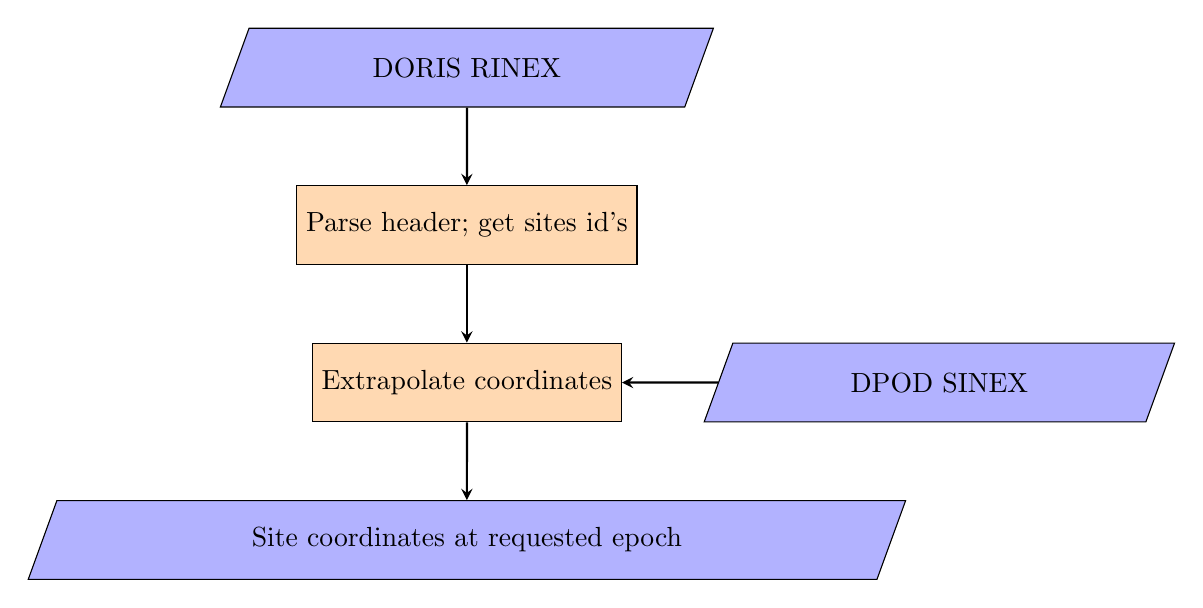
\begin{tikzpicture}[node distance=2cm]
\node (rnxin) [io] {DORIS RINEX};
\node (parsehdr) [process, below of=rnxin] {Parse header; get sites id's};
\node (xtrapolate) [process, below of=parsehdr] {Extrapolate coordinates};
\node (snxin) [io, right of=xtrapolate, xshift=4cm] {DPOD SINEX};
\node (out1) [io, below of=xtrapolate] {Site coordinates at requested epoch};
\draw [arrow] (rnxin) -- (parsehdr);
\draw [arrow] (parsehdr) -- (xtrapolate);
\draw [arrow] (snxin) -- (xtrapolate);
\draw [arrow] (xtrapolate) -- (out1);
\end{tikzpicture}

\section{DPOD}
For the analysis of DORIS observations, we need to have (at least approximate) 
site coordinates for the observed DORIS sites/beacons. Note that in DORIS RINEX 
v3 format \cite{DORISRNX3}, the RINEX files record all the observed sites at the 
file header, using the fields (among others):
\begin{itemize}
    \item 4-character station code,
    \item Station name (\textit{max 30characters long}) and 
    \item DOMES number
\end{itemize}

Example:
\begin{verbatim}
    51                                                      # OF STATIONS
D01  AMVB AMSTERDAM                     91401S005  3   0    STATION REFERENCE
D02  MAUB MARION ISLAND                 30313S005  3   0    STATION REFERENCE
...
D50  BADB BADARY                        12338S002  3   0    STATION REFERENCE 
D51  GRFB GREENBELT                     40451S178  3   0    STATION REFERENCE
\end{verbatim}

To match the sites with external sources (e.g. SINEX files), we will normally use 
the 4-character station code and/or the domes number.

In the meeting on the 15\textsuperscript{th} October 2021, it was suggested that instead of ITRF(2014, ...) 
we should better use the IDS published DPOD set of coordinates/veclocities (for better 
consistency). PDOP is a ``DORIS extension of the ITRF for Precise Orbit Determination'' 
estimated and delivered by the IDS Combination Center; details can be found on the 
\href{https://ids-doris.org/analysis-coordination/combination/dpod.html}{IDS DPOD webpage}.

Currently (October 2021) the latest PDOP realization is DPOD2014 \cite{Moreaux2019118} and 
the latest release is ``August 2020 - version \#5 - \textbf{dpod2014\_0}'' \cite{Moreaux2020};
the corresponding information files are published by 
\href{ftp://cddis.gsfc.nasa.gov/pub/doris/products/dpod/dpod2014/}{cddis} and
\href{ftp://doris.ensg.ign.fr/pub/doris/products/dpod/dpod2014/}{ign} in both 
SINEX and ascii/text format. Of the two, we are going to use the SINEX files (since 
they are more comprehensive, self-contained, capable of holding much more detailed information 
and widely used is Satellite Geodesy). 

Appropriate source code is written so as to be able to read and parse the DPOD SINEX 
file(s) and extrapolate site coordinates to a desired epoch. The sites we want to 
extrapolate coordinates for, are distinguished via their 4character id.

\section{Todo}
\subsection{Coordinate Std Deviations}
Also compute (extrapolated) coordinate stdandard deviations to go with the computed coordinate components.

\subsection{Ignored SINEX Sections}
The \textbf{dpod2014\_0} SINEX file contains a couple of blocks that (at this point) are 
not considered when parsing/extrapolating. These are (\cite{Moreaux2020}):
\begin{itemize}
    \item SOLUTION/DISCONTINUITY: origin (ex: earthquake, beacon change, antenna problem...) of
the position discontinuities
    \item SOLUTION/DATA\_REJECT: periods of time not included in the combination
    \item STATION/TO\_BE\_UPDATED: stations with non-negligible position change wrt DPOD2014v03
\end{itemize}

These are not crucial at this point but should be considered further on.

\section{Technicalities}

Main source code for the above is developed within the 
\begin{itemize}
    \item \href{https://github.com/xanthospap/libsinex}{sinex} and
    \item \href{https://github.com/xanthospap/doris}{doris}
\end{itemize}
repositories.

%The main function that does the work, is:
%\begin{lstlisting}
%#if __cplusplus >= 202002L
%template <typename T>
%    requires(T::is_of_sec_type && !std::is_same_v<T, dso::microseconds>)
%#else
%template <class T,
%          typename = std::enable_if_t<(T::is_of_sec_type) &&
%                                      (!std::is_same_v<T, dso::microseconds>)>>
%#endif
%int extrapolate_sinex_coordinates(
%            const char *snx_fn, char **site_ids, int num_sites,
%            const dso::datetime<T> &t) noexcept {
%    dso::datetime<dso::microseconds> t_micro =
%    t.template cast_to<dso::microseconds>();
%return extrapolate_sinex_coordinates(snx_fn, site_ids, num_sites, t_micro);
%}
%\end{lstlisting}

The following example (\href{https://github.com/xanthospap/doris/blob/main/test/test\_pdop\_crd.cc}{test\_pdop\_crd.cc}) 
extrapolates the coordinates of all the sites recorded in a DORIS RINEX file using a DPOD 
SINEX file. It is tested with the following SINEX files:
\begin{itemize}
    \item dpod2014\_053.snx
\end{itemize}

%\codelst{source/test_pdop_crd.cc}
\chapter{DORIS Ground Segment}
\label{ch:doris-ground-segment}

\tikzset{cross/.style={cross out, draw=red, minimum size=2*(#1-\pgflinewidth), inner sep=0pt, outer sep=0pt},
%default radius will be 1pt. 
cross/.default={1pt}}

\section{Geometry of Ground Antennae}
DORIS observations are referred to the electronic reference point (RP) of the antenna, 
the points where the DORIS observations  are  acquired.  As  that  electronic  point 
(\SI{2}{\GHz} center of phase for DORIS) is virtual and as for example it may change 
while using another type of antenna data referring to that electronic point are of no 
use for geophysical studies. So, observations must be referred to the conventional RP 
which is defined according to the geometry of the antenna. Therefore, one has also to 
account for the distance between the electronic RP and the conventional RP of the antenna (\cite{TOURAIN2016}). 
The ability to get accurate DORIS data relies for one part on the capability of providing 
accurate models to connect the  electronic RP (or electronic phase center) and the conventional 
RP, as well as, phase center variations (\gls{pcv}s) as a function of the elevation angle and azimuth.

The type of antenna is identified by the 4\textsubscript{th} character of the beacon 
mnemonic: letter ``A'' for the Alcatel type; letter ``B'' or letter ``C'' for the 
Starec B or C type.  That is, in the DORIS RINEX field ``STATION REFERENCE'', the 
last character of the second column (aka ``4-character station code''), defines the 
ground beacon antenna type; example:
\begin{Verbatim}[commandchars=\\\{\}]
    51                                                      # OF STATIONS       
D01  BEM\textcolor{red}{B} BELGRANO                      66018S002  3   0    STATION REFERENCE   
D02  ADH\textcolor{red}{C} TERRE ADELIE                  91501S005  3   0    STATION REFERENCE   
D03  SYQ\textcolor{red}{B} SYOWA                         66006S005  3   0    STATION REFERENCE   
D04  CRQ\textcolor{red}{C} CROZET                        91301S004  4   0    STATION REFERENCE   
D05  DIO\textcolor{red}{B} DIONYSOS                      12602S012  3   0    STATION REFERENCE
\end{Verbatim}

\begin{table}[h!]
    \centering
    \begin{tabular}{|c | c | c | c | c|}
        \hline
        Zenith Distance & \multicolumn{2}{c}{ALCATEL (dBi)} & \multicolumn{2}{c|}{STAREC (dBi)} \\
                        & \SI{401.25}{\mega\hertz} & \SI{2036.25}{\mega\hertz} &  \SI{401.25}{\mega\hertz} & \SI{2036.25}{\mega\hertz}\\
        \hline
        \ang{0}&3.2&2.1&3.5&0 \\
        \ang{10}&3.5&2.6&3.6&0.4\\
        \ang{20}&4&2&3.7&0.5\\
        \ang{30}&4.4&4&3.8&1.5\\
        \ang{40}&4.6&4.4&3.7&3.2\\
        \ang{50}&4.2&4.6&3.2&3.9\\
        \ang{60}&2.7&2.7&2.5&4\\
        \ang{70}&0.6&-0.1&1&3.2\\
        \ang{80}&-2.7&-3.3&-1.3&0.2\\
        \ang{90}&-6&-7&-4.2&-5.6\\
        \hline
    \end{tabular}
    \caption{DORIS ground antennae gains, \cite{DORISGSM}.}
    \label{table:antenna-gains}
\end{table}

\subsection{Phase Center Offsets}

Depending on the antenna type, appropriate \gls{pco}s need to be applied to 
the observed quantities for the reduction of the observation vector to the Reference Point 
(from the respective ``virtual'' phase center) of the antenna. When a linear combination 
of the observed quantities is used, a respective \gls{pco} needs to be computed and 
applied. E.g., for the case of the Ionospheric-free linear combination, the respective 
\gls{pco} is:
\begin{equation}
    \vec{r}_{2GHz,iono-free} = \frac{\vec{r}_{400MHz,2GHz}}{\gamma - 1}
\end{equation}

where $\vec{r}_{2GHz,iono-free}$ is the vector from the \SI{2}{\GHz} phase
center to the iono-free phase center and $\vec{r}_{400MHz,2GHz}$ is
the vector from the \SI{400}{MHz} to the \SI{2}{\GHz} phase center.

\begin{table}[h!]
    \centering
    \begin{tabular}{|c|c|c|}
        \hline
        Antenna Type & ALCATEL & STAREC-B \& STAREC-C \\
        \hline
        $\Delta h$ in \si{\mm} for \SI{2}{\GHz} & \SI{510}{\mm} & \SI{487}{\mm}\\
        $\Delta h$ in \si{\mm} for \SI{400}{\MHz} & \SI{335}{\mm} & \SI{0}{\mm}\\
        \hline
    \end{tabular}
    \caption{DORIS ground antennae Phase Center Offsets, \cite{DORISGSM}.}
    \label{table:antenna-pco}
\end{table}

\subsection{DORIS ALCATEL Antenna}

\begin{figure}
\centering
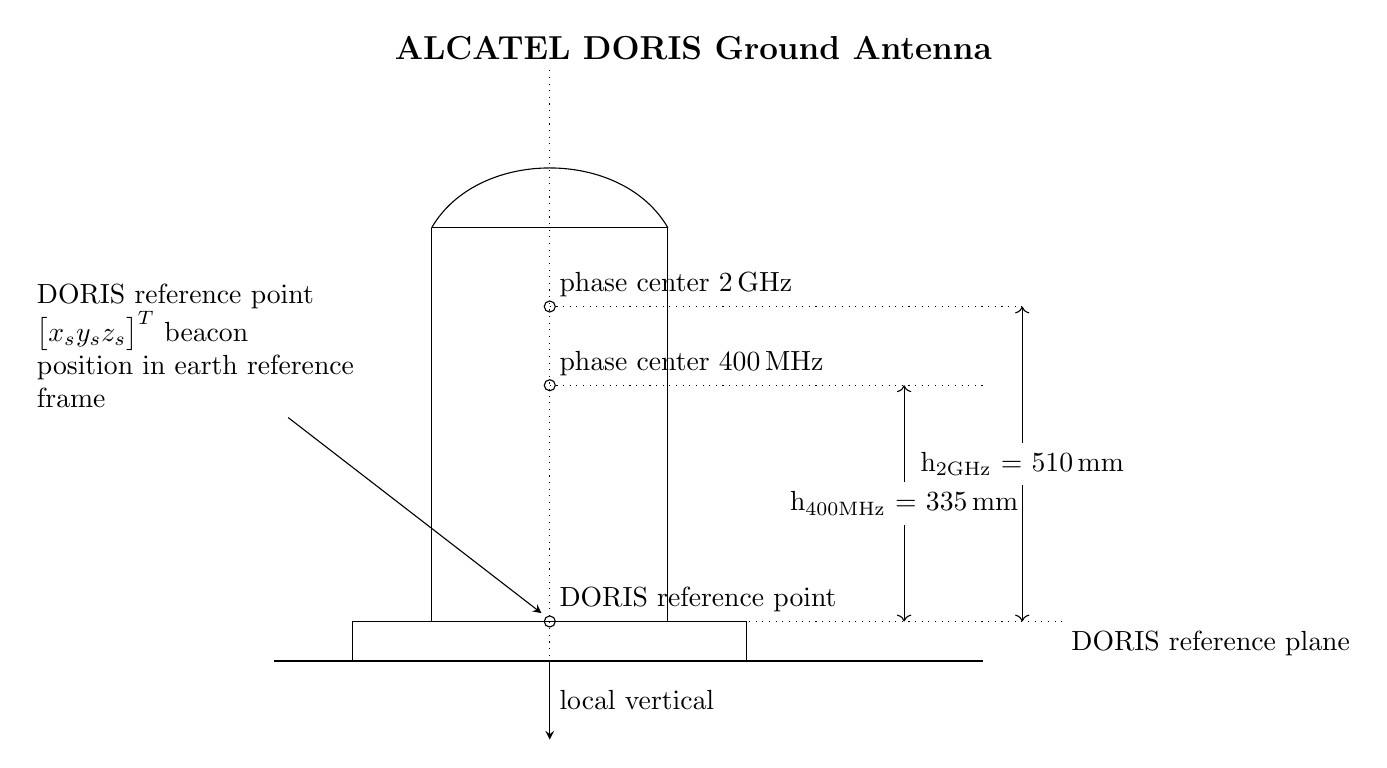
\begin{tikzpicture}
    \draw (2,-2) -- (2,-7); %% left vertical
    \coordinate (LT) at (2,-2);
    \draw (5,-2) -- (5,-7); %% right vertical
    \coordinate (RT) at (5,-2);
    \coordinate (L2PC) at (3.5, -4.0);
    \coordinate (L1PC) at (3.5, -3.0);
    \coordinate (BRP) at (3.5, -7.0);
    \draw (LT) to[out=60, in=120] (RT); %% dome
    \draw (LT) to (RT); %% top horizontal (under dome)
    \draw (1,-7) -- (6,-7); %% reference plain
    \draw (1, -7) -- (1, -7.5); %% left minor vertical
    \draw (6, -7) -- (6, -7.5); %% right minor vertical
    \draw [line width=0.25mm] (0,-7.5) -- (9,-7.5); %% ground
    \draw [-stealth] (3.5,-7.5) --node[anchor=west]{local vertical} (3.5, -8.5); %% local vertical to ground
    \draw [dotted] (3.5, 0) -- (3.5, -7.5); %% local vertical from dome
    
    \draw (L1PC) circle (2pt) node[anchor=south west]{phase center \SI{2}{\GHz}}; %% 2GHz pc
    \draw (L1PC) node[cross=3pt, rotate=0] {}; %% 2GHz cross
    \draw [dotted] (L1PC) -- (9.5, -3.0); %% horizontal from 2GHz PC
    \path (9.5, -7.0) -- node[](hl1){h\textsubscript{2GHz} = \SI{510}{\mm}} (9.5, -3.0);
    \draw [<-] (9.5, -7.0)--(hl1); \draw [->] (hl1)--(9.5, -3.0);
    
    \draw (L2PC) circle (2pt) node[anchor=south west]{phase center \SI{400}{\MHz}}; %% 400 MHz pc
    \draw (L2PC) node[cross=3pt, rotate=0] {}; %% 400MHz cross
    \draw [dotted] (L2PC) -- (9, -4.0); %% horizontal from 400MHz PC
    \path (8, -7.0) -- node[](hl2){h\textsubscript{400MHz} = \SI{335}{\mm}} (8, -4.0);
    \draw [<-] (8, -7.0)--(hl2); \draw[->] (hl2)--(8, -4.0);
    
    \draw (BRP) circle (2pt) node[anchor=south west]{DORIS reference point}; %% reference point
    \draw (BRP) node[cross=3pt, rotate=0] {}; %% RP cross
    \draw [dotted] (BRP) -- (10, -7.0); %% horizontal from RP
    \draw (10, -7) node[anchor=north west]{DORIS reference plane};
    
    \node[rectangle, align=left] (rptext) at (-1,-3.5) {DORIS reference point \\ \(\begin{bmatrix} x_s y_s z_s \end{bmatrix}^{T} \) beacon \\position in earth reference \\frame};
    \draw [-stealth] (rptext) to ($(BRP)-(3pt,-3pt)$);
    \node[above,font=\large\bfseries] at (current bounding box.north) {ALCATEL DORIS Ground Antenna};
\end{tikzpicture}
\caption{Geometry of Alcatel DORIS Ground Antenna/Beacon}
\label{fig:alcatel-antenna}
\end{figure}


\subsection{DORIS STAREC Antenna}
STAREC antennae B and C are identical in terms of design and specification, the
difference is about the error budget in phase center position. For STAREC-C,
manufacturing process and error budget have been improved \cite{DORISGSM}.

According to \cite{TOURAIN2016}, in order to check the consistency of the theoretical 
characteristics of this type of antennae, a measurement campaign was performedby 
the CNES at the Compact Antenna Test Range (CATR). The CATR is a dedicated facility 
consisting ofan anechoic chamber equipped with several specific devices 
allowing significant measurement for satellite characterization.

As a result of the campaign, a phase law was established by averaging the estimated 
phase law values obtained during the CATR characterization. The resulting couple phase 
center position–phase law correction was provided to the  DORIS  users  through  a  
text  file  in  \gls{antex} (\cite{ANTEXv14}) format, available on the IDS website
\url{ftp://ftp.ids-doris.org/pub/ids/stations/doris_phase_law_antex_starec.txt}.

STAREC antennae B and C are identical in terms of design and specification, the
difference is about the error budget in phase center position. For STAREC C,
manufacturing process and error budget have been improved (\cite{DORISGSM}).

\begin{figure}
\centering
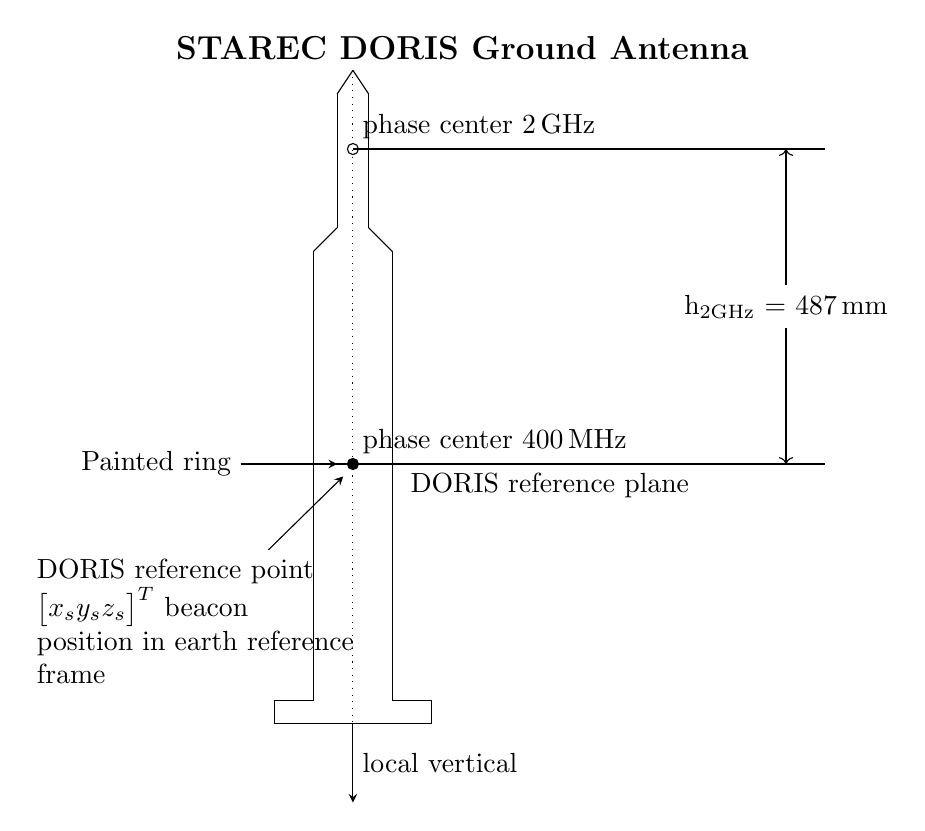
\begin{tikzpicture}
    \coordinate (top) at (4,-1);
    \coordinate (tl) at (3.8, -1.3);
    \coordinate (tr) at (4.2, -1.3);
    \coordinate (blt) at (3.8, -3.0);
    \coordinate (brt) at (4.2, -3.0);
    \coordinate (blb) at (3.5, -3.3);
    \coordinate (brb) at (4.5, -3.3);
    \draw (top) to (tl);
    \draw (tl) to (blt);
    \draw (blt) to (blb);
    \draw (top) to (tr);
    \draw (tr) to (brt);
    \draw (brt) to (brb);
    \draw (blb) to (3.5, -9);
    \draw (brb) to (4.5, -9);
    \draw (3.5, -9) to (3.0, -9);
    \draw (3.0, -9) to (3.0, -9.3);
    \draw (4.5, -9) to (5.0, -9);
    \draw (5.0, -9) to (5.0, -9.3);
    \draw (3.0, -9.3) to (5.0, -9.3);

    \draw [dotted] (top) -- (4.0, -9.3); %% local vertical from top
    \draw [-stealth] (4.0, -9.3) -- node[anchor=west]{local vertical} (4.0, -10.3); %% local vertical arrow

    \coordinate (l1pc) at (4, -2.0);
    \draw (l1pc) circle (2pt) node[anchor=south west]{phase center \SI{2}{\GHz}}; %% 2GHz pc
    \draw (l1pc) node[cross=3pt, rotate=0] {}; %% 2GHz cross
    \draw (l1pc) to (10, -2.0);
    
    \coordinate (l2pc) at (4, -6.0);
    \draw [fill=black] (l2pc) circle (2pt) node[anchor=south west]{phase center \SI{400}{\MHz}}; %% 400MHz pc
    \draw (l2pc) node[cross=3pt, rotate=0] {}; %% 400MHz cross
    \draw ($(l2pc)-(1.0,0.0)$) -- node[below]{DORIS reference plane} (10, -6.0);
    \node (prt) at ($(l2pc)-(2.5,0.0)$) {Painted ring}; 
    \draw [-stealth] (prt) to ($(l2pc)-(0.2,0.0)$);

    \path ($(l1pc)+(5.5, 0.0)$) -- node[](h2g){h\textsubscript{2GHz} = \SI{487}{\mm}} ($(l2pc)+(5.5, 0.0)$);
    \draw [<-] ($(l1pc)+(5.5, 0.0)$) -- (h2g); \draw [->] (h2g) -- ($(l2pc)+(5.5, 0.0)$);

    \node[rectangle, align=left] (rptext) at ($(l2pc)-(2.0,2.0)$) {DORIS reference point \\ \(\begin{bmatrix} x_s y_s z_s \end{bmatrix}^{T} \) beacon \\position in earth reference \\frame};
    \draw [-stealth] (rptext) to ($(l2pc)-(3.5pt,4.5pt)$);

    \node[above,font=\large\bfseries] at (current bounding box.north) {STAREC DORIS Ground Antenna};
\end{tikzpicture}
\caption{Geometry of Alcatel STAREC Ground Antenna/Beacon}
\label{fig:starec-antenna}
\end{figure}

\section{Phase Law}

%\begin{figure}
%\begin{subfigure}{0.45\textwidth}
%  \centering
%  \includegraphics[width=.65\linewidth, angle=-90]{alcatel-phlaw}  
%  \caption{\scriptsize ALCATEL DORIS Ground Antenna Phase Law}
%  \label{fig:pcv-alcatel}
%\end{subfigure}
%\begin{subfigure}{0.45\textwidth}
%  \centering
%  \includegraphics[width=.65\linewidth, angle=-90]{starecbc-phlaw}  
%  \caption{\scriptsize STAREC B/C DORIS Ground Antenna Phase Law}
%  \label{fig:pcv-starec}
%\end{subfigure}
%\caption{DORIS Ground Antenna Phase Law}
%\label{fig:ground-antenna-phase-law}
%\end{figure}
\chapter{Satellite Orbits}
\label{ch:satellite-orbits}

\section{Geopotential}
For precise orbit determination, we need to drop the assumption of the total mass 
of the Earth being concentrated in the center of the coordinate system. For the
following discussion of a more realistic model is adopted, where it is convenient 
to use an equivalent representation involving the gradient of the corresponding 
gravity potential \(U\)
\begin{equation}
    \ddot{\vec{r}} = \nabla U \textrm{ where } U = G M_{\Earth} \frac{1}{r}
\end{equation}

This expression for the potential may easily be generalized to an arbitrary mass
distribution by summing up the contributions created by individual mass elements
\(dm = \rho(\vec{s}) d^3 \vec{s}\) according to (\cite{Montenbruck2000})
\begin{equation}
    U = G \int{\frac{\rho(\vec{s}) d^3 \vec{s}}{\lvert \vec{r} - \vec{s} \rvert}}
\end{equation}

For computations, the Earth's gravity potential at point \((\phi , \lambda)\) 
can be approximated using a spherical harmonics expansion 
(e.g. \cite{Montenbruck2000})
\begin{equation}
    U = \frac{G M_{\Earth}}{r} \sum_{n=0}^\infty \sum_{m=0}^n 
    \frac{R_{\Earth}^n}{r^n} P_{nm}(sin\phi) 
    (C_{nm} cos(m\lambda) + S_{nm} sin(m\lambda))
\end{equation}

with the coefficients \(C_{nm}\) and \(S_{nm}\) describing the dependence on the 
Earth's internal mass distribution. These coefficients can be extracted from a 
suitable  \emph{geopotential model}.

Note that Geopotential coefficients with \(m=0\) are called  \emph{zonal} coefficients, 
since they describe the part of the potential that does not depend on the longitude. 
All \(S_{n0}\) vanish due to their definition, and the notation \(J_n = -C_{n0}\) 
is commonly used for the remaining zonal terms. The other geopotential coefficients
are known as \emph{tesseral} and \emph{sectorial} coefficients for \(m<n\) and 
\(m = n\), respectively.

\fbox{\begin{minipage}{.9\textwidth}
To compute the acceleration \(\ddot{\vec{r}}\), which is equal to the 
gradient of \(U\), we use the recursion formulas described in \cite{Montenbruck2000}.
Note that these expressions, use the \underline{non-normalized} harmonic 
coefficients. 
\end{minipage}}

\subsection{Gravity Models}
The \href{http://icgem.gfz-potsdam.de/home}{International Centre for Global Earth Models (ICGEM)}  
(\cite{icgempub}) web service hosts a large number of gravity field models, 
published in what is called the \emph{The ICGEM-format}(\cite{ICGEMFormat}). 

Such static model files can be parsed and the respective harmonic coeefficients 
(\(C_{nm}\) and \(S_{nm}\)) be used to compute satellite acceleration induced by 
the geopotential.

\section{Sun and Moon Perturbing Acceleration}
According to Newton's law of gravity, the acceleration of a satellite by a point 
mass \(M\) is given by:
\begin{equation}
    \label{eq:mon335}
    \ddot{\vec{r}} = G M \frac{\vec{s}-\vec{r}}{\lvert \vec{s} - \vec{r} \rvert ^3}
\end{equation}
where \(\vec{r}\) and \(\vec{s}\) are the geocentric coordinates of the satellite 
and of \(M\) respectively. Some care is required, however, before this expression 
can be used for describing the satellite's motion with respect to the center of 
the Earth. The value of \(\ddot{\vec{r}}\) in \ref{eq:mon335} refers to an 
inertial or Newtonian coordinate system in which the Earth is not at rest, but 
is itself subject to an acceleration
\begin{equation}
    \ddot{\vec{r}} = G M \frac{\vec{s}}{\lvert \vec{s} \rvert ^3}
\end{equation}
due to M. Both values have to be subtracted to obtain the second derivative
\begin{equation}
    \label{eq:mon337}
    \ddot{\vec{r}} = G M (\frac{\vec{s}-\vec{r}}{\lvert \vec{s} - \vec{r} \rvert ^3} - \frac{\vec{s}}{\lvert \vec{s} \rvert ^3})
\end{equation}
of the satellite's Earth-centered position vector.

\subsection{Sun, Moon and Planetary Ephemerides}
To use the formula \ref{eq:mon337} we need the (geocentric) coordinates of the 
Sun and Moon. To that end, we can either use low-precision solar and lunar 
coordinates (as described e.g. in \cite{Montenbruck2000} and \cite{Vallado}) or 
use JPL Ephemerides. Both options are available.

\subsubsection{JPL Ephemerides}
Jet Propulsion Laboratory Development Ephemeris (abbreved JPL DE(number), or 
simply DE(number)) designates one of a series of mathematical models of the 
Solar System produced at the \href{https://www.jpl.nasa.gov/}{Jet Propulsion Laboratory} 
for use in spacecraft navigation and astronomy. The models consist of numeric 
representations of positions, velocities and accelerations of major Solar System 
bodies, tabulated at equally spaced intervals of time, covering a specified 
span of years (\cite{wiki-jplde}). Further information and a description of 
vailable ephemerides, can be found at the 
\href{https://ssd.jpl.nasa.gov/planets/eph_export.html}{JPL Planetary and Lunar Ephemerides} website.

We use an interface to the JPL-provided Observation Geometry System
for Space Science Missions (\href{https://naif.jpl.nasa.gov/naif/}{SPICE}) 
software library \footnote{based on the C version of the the 
\href{https://naif.jpl.nasa.gov/naif/toolkit_C.html}{Navigation and Ancillary Information facilty}} 
to extract planet coordinates. 

\section{Atmospheric Drag}
Next to the oblateness of the Earth, atmospheric drag most strongly influences the
motion of a satellite near Earth; in fact, during the last few revolutions of the satellite's
life, drag effects can be more dominant than those from the Earth's oblateness. For more
distant satellites, third-body effects and solar-radiation pressure dominate more than
oblateness and drag (\cite{Vallado}). Atmospheric forces represent the largest 
non-gravitational perturbations acting on low altitude satellites.

The cause of drag is the atmospheric particles, which retard the satellite's motion.
Calculating density is extremely complex for real-world problems.

\subsection{Acceleration Due to Drag}
The basic equation for aerodynamic drag combines several factors; I'm showing it here
as a specific force or acceleration (\cite{Vallado}):
\begin{equation}
    \label{eq:val828}
    \ddot{\vec{r}} = -\frac{1}{2} \frac{c_D A}{m} \rho 
    \dot{\vec{r_{rel}}^2} 
    \frac{\dot{\vec{r_{rel}}}}{\lvert \dot{\vec{r_{rel}}} \rvert}
\end{equation}

where:
\begin{itemize}
    \item \(c_D\) is the coefficient of drag; a dimensionless quantity which reflects 
    the satellite's susceptibility to drag forces. 
    \item \(\rho\) is the atmospheric density which indicates how dense the atmosphere 
    is at the satellite altitude and is perhaps the most difficult parameter to determine.
    \item \(A\) is the cross-sectional area, defined to be the area which is normal 
    to the satellite's velocity vector.
    \item \(m/(c_D A)\) is called the ballistic coefficient.
\end{itemize}
The direction of the drag acceleration is always (anti-)parallel to the relative 
velocity vector, indicated by the unit vector 
\(\vec{e_u} = \dot{\vec{r_{rel}}} / \lvert \dot{\vec{r_{rel}}} \rvert \)

Note that in \ref{eq:val828}, \(\vec{r_{rel}}\) is not the velocity vector 
typically found in the state vector. This velocity vector is relative to the 
atmosphere, which depends on complex atmospheric dynamics. However, a reasonable 
approximation of the relative velocity is obtained with the assumption that the 
atmosphere co-rotates with the Earth:
\begin{equation}
    %\begin{align}
    \dot{\vec{r_{rel}}} = \frac{d\vec{r}}{dt} - \vec{\omega}_{\Earth} \times \vec{r} = 
        \begin{bmatrix}
        \frac{dx}{dt}+{\omega}_{\Earth}y \\
        \frac{dy}{dt}-{\omega}_{\Earth}x \\
        \frac{dz}{dt}
        \end{bmatrix}
    %\end{align} 
\end{equation}
with the inertial satellite velocity vector \(d\vec{r}/{dt}\), the position vector 
\(\vec{r}\), and the Earth's angular velocity vector \(\vec{\omega}_{\Earth}\). 
As the drag force depends on the atmospheric density \(\rho\) at the satellite 
location, the modeling of the complex properties and dynamics of the Earth's 
atmosphere is a challenging task of modern precision orbit determination.

\subsection{Magnetic Field Models}
The effect of the magnetic variations of the Earth and Sun is useful with calculations of
atmospheric density because it's believed that magnetic variations are related to fluctua-
tions in atmospheric density. The charged particles from any magnetic disturbances cause ionization in the upper atmosphere,
thereby affecting the density and, subsequently, the drag. \ul{The effects of
drag resulting from magnetic disturbances are noticeable for satellites at altitudes
between 300 km and 1000 km} (\cite{Vallado}).

\subsection{Solar Flux}
The contribution of solar flux to atmospheric density is mainly from incoming solar
radiation. Solar flux (or Extreme Ultra-Violet, EUV, radiation that heats the upper
atmosphere, \(F_{EUV}\). Solar flux receives a lot of attention because it is an important parameter in determining
atmospheric density. The primary quantity, \(F_{10.7}\), has been used as a proxy for the EUV
radiation for many years.

\subsection{Model Atmospheres}
Numerous density models have been developed over the past few decades to find density, 
both static and time-varying, to satisfy differing accuracy models.
\begin{itemize}
    \item \emph{Exponential Model (0-1000 km)}, simple, static model assumes the density of the atmosphere decays exponentially
    with increasing altitude.
    \item \emph{NRLMSIS-00 (0-2000 km)}\cite{nrlmsise00}, quite accurate and has been successfully applied to many stressing problems.
\end{itemize}

\chapter{Orbit Integrators}
\label{ch:orbit-integrators}

\section{Introduction}
Determination and prediction of orbits requires an orbit propagator that finds the
phase space state of a satellite at one time based on its state at another time.
An \gls{ode} of order \( n \) is an equation of the form:
\begin{equation}
	\frac{d^n y}{dt^n} = f(t,y,y',y'',\ldots,y^{n-1})
\end{equation}
Initial value problems involving higher-order \glspl{ode} require initial conditions 
for each derivative through \( y^{n-1} \). 
The solution to an initial value problem, \( y(t) \) most often must be found numerically;
algorithms that numerically solve initial value problems are known as \emph{numerical integrators}.

Higher-order \glspl{ode} may be transformed to an equivelent set of 1\textsuperscript{st} 
order equations and be solved with a standard numerical integrator; however, some 
numerical integrators are designed to directly solve higher-order \glspl{ode}.

\emph{Multi-step integrators} (also called \emph{predictor-corrector} methods) 
integrate forward from a particular time to the next mesh
point using function values at the current point as well as several previous mesh
points. The set of the previous points used as well as the current point is called the
set of \emph{backpoints} (\cite{berry2004}). The methods develop a Taylor series 
in the time separation between mesh points, and this series must be truncated after 
some number of terms, which thereby gives the \emph{order} of the method. The order is one 
less than the number of backpoints, and is not related to the order of the differential equation.
There a re various multi-step integrators, depending on the implementation.

The function \( f(t,y) \) must be continuous and smooth through the set of 
backpoints. If there are any discontinuities in \( f \), for example going through eclipse when 
solar radiation pressure is considered, the integration must either be restarted, or 
modified to handle the discontinuity (\cite{berry2004}).

\section{Difference Tables}
Predictor-corrector integrators can be defined in terms of difference tables. 
For a fixed-step method, assume that solution values \( y_n \) are known on a 
discrete set of equally-spaced mesh points 
\( \ldots, t_0 - 2h , t_0 - h , t_0 , t_0 + h , t_0 + 2h , \ldots \)
where \( h \) is the \emph{step}. If we define \(  t_n \equiv t_0 + n h \), then the 
set of points is \( t_{-2}, t_{-1}, t_0 , t_{1}, t_{2} \) with the corrsponding 
function values \( f_n = f(t_n , y_n ) \), where \( y_n \) is the numerical solution 
at the mesh point \( t_n \).

There are three kinds of differences \footnote{Note that a more general backward difference formula, 
reads:
\begin{equation}
  \begin{aligned}
    & \text{\textbf{forward differene} } {\Delta}_h [f](x) = f(x+h) - f(x)\\  
    & \text{\textbf{backward difference} } {\nabla}_h [f](x) = f(x) - f(x-h) = {\Delta}_h [f](x-h)\\
    & \text{\textbf{central difference} } {\delta}_h [f](x) = f(x+\frac{h}{2}) - f(x-\frac{h}{2}) = {\Delta}_{h/2} [f](x) + {\nabla}_{h/2} [f](x)\\
  \end{aligned}
\end{equation}
When the step size \( h \) is ommited, it is taken to be \(1\). }, 
represented by different operators (following \cite{berry2004}):
\begin{equation}
  \begin{aligned}
    \text{forward differene     } &   \Delta f_i    = & f_{i+1} - f_i \\
    \text{backward difference    } & \nabla f_i  = & f_i - f_{i-1} \\
    \text{central difference    } &   \delta f_i   = & f_{i+1/2} - f_{i-1/2} \\
  \end{aligned}
\end{equation}

The differences of the
differences, or \emph{second differences}, can also be computed. For instance,
the square of the backward difference operator is the operator applied to the first
difference \footnote{
  On a more genral manner, the n\textsuperscript{th} order forward, backward and central differences read :
\begin{equation}
  \begin{aligned}
  & {\Delta}^n_h [f](x) = \sum_{k=0}^n \binom{n}{k} (-1)^{n-k} f(x+k)\\
  & {\nabla}^n_h [f](x) = \sum_{i=0}^n (-1)^i \binom{n}{i} f(x-ih)\\
  & {\delta}^n_h [f](x) = \sum_{i=0}^n (-1)^i \binom{n}{i} f(x + (\frac{n}{2} -i)h)\\
  \end{aligned}
\end{equation}
respectively.}
\begin{equation}
  {\nabla}^2 f_i = \nabla \nabla f_i = \nabla (f_i - f_{i-1}) = 
  (f_i - f_{i-1}) - (f_{i-1} - f_{i-2}) = f_i - 2 f_{i-1} + f_{i-2}
\end{equation}

In addition to the three difference operators, there is also a 
\emph{displacement operator} \(E\). The displacement operator is defined as:
\begin{equation}
  E f_i = f_{i+1} \text{ and } E^n f_i = f_{i+n}
\end{equation}

The difference and displacement operators  can be written in terms of each other:
\begin{equation}
  \nabla = 1 - E^{-1} \text{ and } E = \frac{1}{1 - \nabla}
\end{equation}

\begin{figure}
\centering
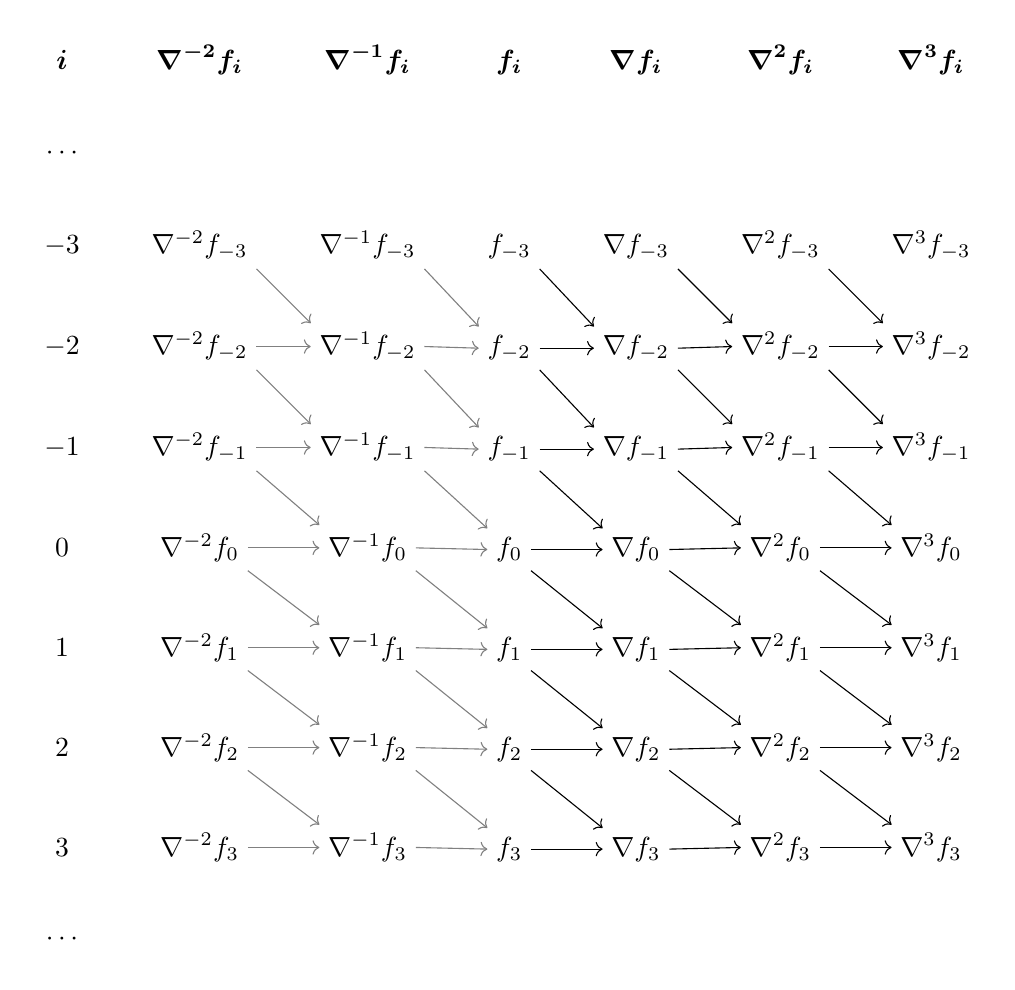
\begin{tikzpicture}
\matrix[
  matrix of math nodes,
  inner sep=3pt,
  row sep=2em,
  column sep=2em
] (M)
{
    \bm{i} & \bm{{\nabla}^{-2} f_i} & \bm{{\nabla}^{-1} f_i} & \bm{f_i} & \bm{\nabla f_i} & \bm{{\nabla}^2 f_i} & \bm{{\nabla}^3 f_i} \\
    \cdots \\
    -3 & {\nabla}^{-2} f_{-3} & {\nabla}^{-1} f_{-3} & f_{-3} &  \nabla f_{-3}  &  {\nabla}^2 f_{-3}  & {\nabla}^3 f_{-3} \\
    -2 & {\nabla}^{-2} f_{-2} & {\nabla}^{-1} f_{-2} & f_{-2} &  \nabla f_{-2}  &  {\nabla}^2 f_{-2}  & {\nabla}^3 f_{-2} \\
    -1 & {\nabla}^{-2} f_{-1} & {\nabla}^{-1} f_{-1} & f_{-1} &  \nabla f_{-1}  &  {\nabla}^2 f_{-1}  & {\nabla}^3 f_{-1} \\
     0 & {\nabla}^{-2} f_{0}  & {\nabla}^{-1} f_{0}  & f_{0}  &  \nabla f_{0}   &  {\nabla}^2 f_{0}   & {\nabla}^3 f_{0}  \\
     1 & {\nabla}^{-2} f_{1}  & {\nabla}^{-1} f_{1}  & f_{1}  &  \nabla f_{1}   &  {\nabla}^2 f_{1}   & {\nabla}^3 f_{1}  \\
     2 & {\nabla}^{-2} f_{2}  & {\nabla}^{-1} f_{2}  & f_{2}  &  \nabla f_{2}   &  {\nabla}^2 f_{2}   & {\nabla}^3 f_{2}  \\
     3 & {\nabla}^{-2} f_{3}  & {\nabla}^{-1} f_{3}  & f_{3}  &  \nabla f_{3}   &  {\nabla}^2 f_{3}   & {\nabla}^3 f_{3}  \\
    \cdots \\
}
;
\draw[->] (M-3-4.south east) -- (M-4-5.north west);
\draw[->] (M-4-4.south east) -- (M-5-5.north west);
\draw[->] (M-5-4.south east) -- (M-6-5.north west);
\draw[->] (M-6-4.south east) -- (M-7-5.north west);
\draw[->] (M-7-4.south east) -- (M-8-5.north west);
\draw[->] (M-8-4.south east) -- (M-9-5.north west);
\draw[->] (M-4-4.east) -- (M-4-5.west);
\draw[->] (M-5-4.east) -- (M-5-5.west);
\draw[->] (M-6-4.east) -- (M-6-5.west);
\draw[->] (M-7-4.east) -- (M-7-5.west);
\draw[->] (M-8-4.east) -- (M-8-5.west);
\draw[->] (M-9-4.east) -- (M-9-5.west);
\draw[->] (M-3-5.south east) -- (M-4-6.north west);
\draw[->] (M-4-5.south east) -- (M-5-6.north west);
\draw[->] (M-5-5.south east) -- (M-6-6.north west);
\draw[->] (M-6-5.south east) -- (M-7-6.north west);
\draw[->] (M-7-5.south east) -- (M-8-6.north west);
\draw[->] (M-8-5.south east) -- (M-9-6.north west);
\draw[->] (M-4-5.east) -- (M-4-6.west);
\draw[->] (M-5-5.east) -- (M-5-6.west);
\draw[->] (M-6-5.east) -- (M-6-6.west);
\draw[->] (M-7-5.east) -- (M-7-6.west);
\draw[->] (M-8-5.east) -- (M-8-6.west);
\draw[->] (M-9-5.east) -- (M-9-6.west);
\draw[->] (M-3-6.south east) -- (M-4-7.north west);
\draw[->] (M-4-6.south east) -- (M-5-7.north west);
\draw[->] (M-5-6.south east) -- (M-6-7.north west);
\draw[->] (M-6-6.south east) -- (M-7-7.north west);
\draw[->] (M-7-6.south east) -- (M-8-7.north west);
\draw[->] (M-8-6.south east) -- (M-9-7.north west);
\draw[->] (M-4-6.east) -- (M-4-7.west);
\draw[->] (M-5-6.east) -- (M-5-7.west);
\draw[->] (M-6-6.east) -- (M-6-7.west);
\draw[->] (M-7-6.east) -- (M-7-7.west);
\draw[->] (M-8-6.east) -- (M-8-7.west);
\draw[->] (M-9-6.east) -- (M-9-7.west);
\draw[gray,->] (M-3-3.south east) -- (M-4-4.north west);
\draw[gray,->] (M-4-3.south east) -- (M-5-4.north west);
\draw[gray,->] (M-5-3.south east) -- (M-6-4.north west);
\draw[gray,->] (M-6-3.south east) -- (M-7-4.north west);
\draw[gray,->] (M-7-3.south east) -- (M-8-4.north west);
\draw[gray,->] (M-8-3.south east) -- (M-9-4.north west);
\draw[gray,->] (M-4-3.east) -- (M-4-4.west);
\draw[gray,->] (M-5-3.east) -- (M-5-4.west);
\draw[gray,->] (M-6-3.east) -- (M-6-4.west);
\draw[gray,->] (M-7-3.east) -- (M-7-4.west);
\draw[gray,->] (M-8-3.east) -- (M-8-4.west);
\draw[gray,->] (M-9-3.east) -- (M-9-4.west);
\draw[gray,->] (M-3-2.south east) -- (M-4-3.north west);
\draw[gray,->] (M-4-2.south east) -- (M-5-3.north west);
\draw[gray,->] (M-5-2.south east) -- (M-6-3.north west);
\draw[gray,->] (M-6-2.south east) -- (M-7-3.north west);
\draw[gray,->] (M-7-2.south east) -- (M-8-3.north west);
\draw[gray,->] (M-8-2.south east) -- (M-9-3.north west);
\draw[gray,->] (M-4-2.east) -- (M-4-3.west);
\draw[gray,->] (M-5-2.east) -- (M-5-3.west);
\draw[gray,->] (M-6-2.east) -- (M-6-3.west);
\draw[gray,->] (M-7-2.east) -- (M-7-3.west);
\draw[gray,->] (M-8-2.east) -- (M-8-3.west);
\draw[gray,->] (M-9-2.east) -- (M-9-3.west);
\end{tikzpicture}
\caption{Backward Difference Table. The arrows in the table point towards the difference; 
the upper component is always subtracted from the lower, e.g. \( {\nabla}^2 f_3 = \nabla f_3 - \nabla f_2\)
\cite{berry2004}.}
\label{fig:differences-table-integrator}
\end{figure}

\chapter{Satellite Orbit modeling}
\label{ch:satellite-orbit-modeling}

\section{Quick Note: The State-Space Notation}
It is often helpfull to represent a linear differential equation in the the
\emph{state-space} form, that is a first-order matrix differential equation of
the form:
\begin{equation}
	\dot{\vec{x}} = \bm{F} \vec{x} + \bm{G} \vec{u} + \vec{w}
\end{equation}

where:
\begin{itemize}
	\item \(\vec{x}\) is the system \emph{state vector},
	\item \(\bm{F}\) is system's \emph{dynamic matrix},
	\item \(\vec{u}\) is a deterministic input, sometimes called a \emph{control vector}, and
	\item \(\vec{w}\) is a random forcing function, which is also known as \emph{process noise}
\end{itemize}

\section{Linearization of the Orbit Determination Process}
In the general orbit determination problem, both the dynamics and the measurements
involve significant nonlinear relationships. For the general case, the governing
relations involve the nonlinear expression:
\begin{subequations}
	\begin{align}
		\dot{\vec{x}} = F( \vec{x}, t ),
		 & \quad \vec{x}(t_k ) \equiv \vec{x}_k
		\label{eq:tapley421} \\
		\vec{y}_i = G( \vec{x}_i , t_i ) + {\epsilon}_i ,
		 & \quad  i=1,2,\ldots ,l
		\label{eq:tapley422}
	\end{align}
\end{subequations}

where \(\vec{x}_k\) is the unknown \(n\)-dimensional state vector at time \(t_k\) and
\(\vec{y}_i\) for \(i=1,2,\ldots ,l\) is a \(p\)-dimensional set of observations. The
\emph{best estimate} of the state vector \(\vec{x}_k\) will be denoted as \(\hat{\vec{x}}_k\).
In general, \(p<n\) and \( m = p \times l \gg n \). The formulation described by the
system \ref{eq:tapley421} and \ref{eq:tapley422}, is characterized by: (\cite{tapley})
\begin{enumerate}
	\item the inability to observe the state (\(\vec{x}_k\)) directly,
	\item nonlinear relations between the observations and the state,
	\item fewer observations at any time epoch \(i\) than there are state vector
	      components (\(p<n\)), and
	\item errors in the observations represented by \({\epsilon}_i\)
\end{enumerate}

If a reasonable reference trajectory \(\vec{x}*\) is available and if
\(\vec{x}\), the true trajectory, and the reference trajectory remain sufficiently
close throughout the time interval of interest, then the trajectory for the actual
motion can be expanded in a Taylor’s series about the reference trajectory at
each point in time. Eliminating higher order terms, the deviation in the state
from the reference trajectory can be described by a set of linear differential
equations. Corresponding linear relations can be derived between the observation
and the state deviations, thus transforming the nonlinear orbit determination problem
to a linear one.

If \(\vec{\delta x}\) is the \( n \times 1 \) state deviation vector and
\(\vec{\delta y}\) is the \(p \times 1\) observation deviation:
\begin{equation}
	\begin{aligned}
		\vec{\delta x} (t) & = \vec{x}(t) - \vec{x}^* (t) \\
		\vec{\delta y} (t) & = \vec{y}(t) - \vec{y}^*(t)
	\end{aligned}
\end{equation}

hence

\begin{equation}
	\dot{\vec{\delta x}} (t) = \dot{\vec{x}} (t) - \dot{\vec{x}}^* (t)
\end{equation}

Expanding \ref{eq:tapley421} and \ref{eq:tapley422} in a Taylor series about the
reference trajectory, leads to:
\begin{equation}
	\label{eq:tapley425}
	\begin{aligned}
		\dot{\vec{x}} (t) & = F (\vec{x}, t) \\
		                  & \approx F (\vec{x}^* , t)
		+ \left.\frac{\partial F(t)}{\partial \vec{x}(t)}\right|_{\vec{x}^*} \left( \vec{x}(t) - \vec{x}^* (t) \right)
		+ O_F \left( \vec{x}(t) - \vec{x}^* (t) \right) \\
		\vec{y}_i         & = G( \vec{x}_i , t_i ) + {\epsilon}_i =        \\ & \approx G( \vec{x}^*_i , t_i )
		+ \left.\frac{\partial G}{\partial \vec{x}}\right|_{\vec{x}^* , i} \left.\left( \vec{x}(t_i) - \vec{x}^* (t_i) \right)\right|_{i}
		+ O_G \left( \vec{x}(t_i) - \vec{x}^* (t_i) \right) + {\epsilon}_i \\
	\end{aligned}
\end{equation}

where \(\left.\frac{\partial}{\partial \vec{x}}\right|_{\vec{x}^*}\) indicates that
the partial derivative matrix is evaluated on the reference solution \(\vec{x}^* (t)\)
which is obtained by integrating \ref{eq:tapley421} with the initial conditions
\(\vec{x}^* (t_0)\). \(O_F\) and \(O_G\) indicate terms higher than the 1\textsuperscript{st}
order which are ignored. Noting that \(\dot{\vec{x}}^* = F(\vec{x}^* ,t)\) and
\(\vec{y}^*_i = G(\vec{x}^*_i , t_i )\), and letting
\begin{subequations}
	\begin{align}
		\delta \vec{x}(t) & = \vec{x}(t) - \vec{x}^*(t) \label{eq:tapley426ua} \\
		\delta \vec{x}_i  & = \vec{x}(t_i) - \vec{x}^*(t_i)\label{eq:tapley426ub} \\
		\delta \vec{y}_i  & = \vec{y}_i - G(\vec{x}^*_i , t_i ) \label{eq:tapley426uc}
	\end{align}
\end{subequations}

\ref{eq:tapley421} can be written as:
\begin{align}
	\label{eq:tapley426a}
	\delta \dot{\vec{x}}(t) & = A(t) \delta \vec{x}(t) \\
	\label{eq:tapley426b}
	\delta \vec{y}_i        & = \tilde{H}_i \delta \vec{x}_i + {\epsilon}_i \quad (i=1,\ldots,l)
\end{align}

where
\begin{equation}
	\label{eq:tapley426ah}
	A(t) = \left.\frac{\partial F(t)}{\partial \vec{x} (t)}\right|_{\vec{x}^*}
	\quad
	\tilde{H}_i = \left.\frac{\partial G}{\partial \vec{x}}\right|_{\vec{x}^* , i}
\end{equation}

\section{State Transition Matrix}
\ref{eq:tapley426a} represents a system of linear differential equations with time-dependent
coefficients; the general solution to the system, can be expressed as:
\begin{equation}
	\label{eq:tapley427}
	\bm{x}(t) = \Phi (t, t_k) \cdot \bm{x}_k \quad \text{with } \bm{x}_k = \bm{x}(t_k)
\end{equation}

The matrix \(\Phi (t_i, t_k) \) is called the \emph{state transition matrix} and has the
following properties:
\begin{itemize}
	\item \(\Phi (t_k, t_k) = I \)
	\item \(\Phi (t_i, t_k) = \Phi (t_i, t_j) \Phi (t_j, t_k) \)
	\item \(\Phi (t_i, t_k) = {\Phi}^{-1} (t_j, t_k) \)
\end{itemize}

Noting that \(\bm{x}_k\) is constant,
\begin{equation}
	\label{eq:tapley429}
	\bm{\dot{x}}(t) = \dot{\Phi} (t, t_k) \cdot \bm{x}_k
\end{equation}

Using \ref{eq:tapley426a} and \ref{eq:tapley427},
\begin{equation}
	\label{eq:tapley4210}
	\begin{aligned}
		\dot{\Phi} (t, t_k) \bm{x}_k & = A(t) \cdot \bm{x} (t) \\
		                             & = A(t) \cdot \Phi (t, t_k) \bm{x}_k \\
		\implies                     & \dot{\Phi} (t, t_k) = A(t) \Phi (t, t_k)
	\end{aligned}
\end{equation}

\ref{eq:tapley4210} represents a linear differential equation. For any practical orbit
determination application, the solution for \(\Phi (t, t_0)\)  will be obtained
via numerical integration, supplying a vector of derivative values for the differential
equation of the nominal state vector and computed values for \(\dot{\Phi} (t, t_0)\).

\section{Observations}
Combining \ref{eq:tapley427} and \ref{eq:tapley426b}, we get:
\begin{equation}
	\label{eq:tapley4237}
	\begin{aligned}
		\bm{y}_0     & = \tilde{H}_0 \Phi (t_0, t_k) \bm{x}_k + {\epsilon}_0 \\
		\bm{y}_1     & = \tilde{H}_1 \Phi (t_1, t_k) \bm{x}_k + {\epsilon}_1  \\
		             & \vdotswithin{=} \\
		\bm{y}_{l-1} & = \tilde{H}_{l-1} \Phi (t_{l-1}, t_k) \bm{x}_k + {\epsilon}_{l-1}
	\end{aligned}
\end{equation}

where the system contains \(m=p\times l\) observations and \(n\) unknown components
in the state vector. For convinience, we define the following notation:
\begin{equation}
	\bm{y} \equiv \begin{bmatrix} y_0 \\ y_1 \\ \ldots \\ y_{l-1} \end{bmatrix},
	\quad
	H \equiv \begin{bmatrix} \tilde{H}_0 \Phi (t_0, t_k) \\ \tilde{H}_1 \Phi (t_1, t_k) \\ \ldots \\ \tilde{H}_{l-1} \Phi (t_{l-1}, t_k) \end{bmatrix},
	\quad
	\bm{\epsilon} \equiv \begin{bmatrix} {\epsilon}_0 \\ {\epsilon}_1 \\ \ldots \\ {\epsilon}_{l-1} \end{bmatrix}
\end{equation}

so that we can now write \ref{eq:tapley4237} as:
\begin{equation}
	\label{eq:tapley4239}
	\bm{y} = H \bm{x} + \bm{\epsilon}
	\quad
	\bm{y} \in \mathbb{R} ^{m \times 1},
	\bm{x} \in \mathbb{R} ^{n \times 1},
	H \in \mathbb{R}^{m \times n},
\end{equation}

where \( m = p \times l \) is the total number of observations.

\section{Sequential Estimation Overview}
In the sequential estimation algorithm, observations are processed as soon as they
are received (in contrast to batch estimation), thus offering the advantage of
inverting a matrix of the same dimension as the observation vector. Hence, if the
observations are processed individually, only scalar divisions will be required to
obtain the estimate of \(\vec{x}_k\). The sequential estimation algorithm discussed
here, is often reffered to as the \emph{Kalman filter}, named after Rudolf E. K\'alm\'an
who was one of the primary developers of its theory.

An estimate \(\hat{\bm{x}}_j \) and a covariance matrix \(P_j\) can be
propagated forward to an epoch \(t_k\) by the relations (known as the
\emph{time update} equations)
\begin{subequations}
	\label{eq:tapley471}
	\begin{align}
		\bar{\bm{x}} _k & = \Phi (t_k, t_j) \hat{\bm{x}}_j
		\label{eq:tapley471a} \\
		\bar{P}_k       & = \Phi (t_k, t_j) P_j \Phi ^T (t_k, t_j)
		\label{eq:tapley471b}
	\end{align}
\end{subequations}


Assume that we have a new, additional obervation at epoch \(t_k\),
\begin{equation}
	\bm{y}_k = \tilde{H}_k \bm{x}_k + \bm{\epsilon} _k ,
	\quad E\left[\bm{\epsilon} _k \right] = 0,
	\quad E\left[\bm{\epsilon} _k \bm{\epsilon} ^T_j \right] = R_k \delta _{kj}
\end{equation}

(where \(\delta _{kj}\) is the \emph{Kronicker delta}). We wish to process
\(\bm{y} _k\) in order to determine \(\hat{\bm{x}} _k\). The best estimate of
\(\bm{x} _k\) is

\begin{equation}
	\label{eq:tapley473}
	\hat{\bm{x}} _k = \left( \tilde{H}^T_k R^{-1}_k \tilde{H}_k + \bar{P}^{-1}_k \right)^{-1} \left( \tilde{H}^T_k R^{-1}_k \bm{y}_k + \bar{P}^{-1}_k \bar{\bm{x}}_k \right)
\end{equation}

\ref{eq:tapley473} implies the inversion of the \(n \times n\) \emph{information matrix} 
(more on the information matrix at \ref{sec:information-matrix-and-information-filter}) \(\Lambda _k\),
\begin{equation}
	\label{eq:tapley474}
	\Lambda ^{-1}_k \equiv P_k =
	\left( \tilde{H}^T_k R^{-1}_k \tilde{H}_k + \bar{P}^{-1}_k \right)^{-1}
\end{equation}

From \ref{eq:tapley474}, it follows that:
\begin{equation}
	\label{eq:tapley475}
	P^{-1}_k
	= \tilde{H}^T_k R^{-1}_k \tilde{H}_k + \bar{P}^{-1}_k
\end{equation}

Premultiplying each side of \ref{eq:tapley475} by \(P_k\) and then postmultiplying
by \(\bar{P}_k\), leads to:
\begin{subequations}
	\begin{align}
		\bar{P}_k & =
		P_k \tilde{H}^T_k R^{-1}_k \tilde{H}_k \bar{P}_k + P_k
		\quad or \label{eq:tapley476} \\
		P_k       & =
		\bar{P}_k - P_k \tilde{H}^T_k R^{-1}_k \tilde{H}_k \bar{P}_k
		\label{eq:tapley477}
	\end{align}
\end{subequations}

Postmultiplying \ref{eq:tapley476} by \(\tilde{H}^T_k R^{-1}_k\)
\begin{equation}
	\label{eq:tapley478}
	\begin{aligned}
		\bar{P}_k \tilde{H}^T_k R^{-1}_k                           & =
		P_k \tilde{H}^T_k R^{-1}_k \tilde{H}_k \bar{P}_k \tilde{H}^T_k R^{-1}_k +
		P_k \tilde{H}^T_k R^{-1}_k                                 &                                     \\
		                                                           & = P_k \tilde{H}^T_k R^{-1}_k \left(
		\tilde{H}_k \bar{P}_k \tilde{H}^T_k R^{-1}_k + I \right)   &                                     \\
		                                                           & = P_k \tilde{H}^T_k R^{-1}_k \left(
		\tilde{H}_k \bar{P}_k \tilde{H}^T_k + R_k \right) R^{-1}_k &
	\end{aligned}
\end{equation}

We can postmultiply \ref{eq:tapley478} by \(R_k\) and then by
\(\left(\tilde{H}_k \bar{P}_k \tilde{H}^T_k + R_k \right) ^{-1} \) to solve for
the quantity \(P_k \tilde{H}^T_k R^{-1}_k\):
\begin{equation}
	\label{eq:tapley479}
	P_k \tilde{H}^T_k R^{-1}_k =
	\bar{P}_k \tilde{H}^T_k \left( \tilde{H}_k \bar{P}_k \tilde{H}^T_k + R_k \right) ^{-1}
\end{equation}

which relates the \emph{a-priori} covariance matrix \(\bar{P}_k\) to the
\emph{a-posteriori} covariance matrix \(P_k\).

Substituting \ref{eq:tapley479} into \ref{eq:tapley477}, yields:
\begin{equation}
	\label{eq:tapley4710}
	P_k =
	\bar{P}_k - \bar{P}_k \tilde{H}^T_k \left( \tilde{H}_k \bar{P}_k \tilde{H}^T_k + R_k \right) ^{-1} \tilde{H}_k \bar{P}_k
\end{equation}

\ref{eq:tapley4710} is an alternate way of computing the inverse in \ref{eq:tapley474},
but here the matrix to be inverted is of dimension \(p \times p\), that is the
same dimensions as the observation error covariance matrix. If the observations are
processed as scalars (i.e. one at a time), only a scalar division is required.

If we define the weighting matrix \(K_k\), usually called \emph{Kalman gain matrix},
as
%\begin{equation}
\begin{tcolorbox}[ams equation]
	\label{eq:tapley4711}
	K_k = \bar{P}_k \tilde{H}^T_k \left( \tilde{H}_k \bar{P}_k \tilde{H}^T_k + R_k \right) ^{-1}
\end{tcolorbox}
%\end{equation}

then \ref{eq:tapley4710} reads
%\begin{equation}
\begin{tcolorbox}[ams equation]
	\label{eq:tapley4712}
	P_k = \left( I - K_k \tilde{H}_k \right) \bar{P}_k
\end{tcolorbox}
%\end{equation}

Note also, that substituting \ref{eq:tapley479} into \ref{eq:tapley4711}, we get
\begin{equation}
	\label{eq:tapley4714}
	K_k = P_k \tilde{H}^T_k R^{-1}_k
\end{equation}

Substituting \ref{eq:tapley474} into \ref{eq:tapley473}, we get:
\begin{equation}
	\begin{aligned}
		\hat{\bm{x}}_k & = P_k
		\left( \tilde{H}^T_k R^{-1}_k \bm{y}_k + \bar{P}^{-1}_k \bar{\bm{x}}_k \right)                                \\
		               & = \underbrace{P_k \tilde{H}^T_k R^{-1}_k}_{K_k} \bm{y}_k + P_k \bar{P}^{-1}_k \bar{\bm{x}}_k \\
		               & = K_k \bm{y}_k + P_k \bar{P}^{-1}_k \bar{\bm{x}}_k                                           \\
		               & = K_k \bm{y}_k + \left( I - K_k \tilde{H}_k \right) \bar{P}_k \bar{P}^{-1}_k \bar{\bm{x}}_k
	\end{aligned}
\end{equation}

and finaly
%\begin{equation}
\begin{tcolorbox}[ams equation]
	\label{eq:tapley4716}
	\hat{\bm{x}}_k = \bar{\bm{x}}_k + K_k \left( \bm{y}_k - \tilde{H}_k \bar{\bm{x}}_k \right)
\end{tcolorbox}
%\end{equation}

\ref{eq:tapley4711}, \ref{eq:tapley4712}, \ref{eq:tapley4716} along with \ref{eq:tapley471} can be used in a recursive fashion to compute the estimate \(\hat{\bm{x}}_k\)
incorporating the observation \(\bm{y}_k\).

\subsection{Sequential Estimation Algorithm}
\label{ssec:sequential-estimation-algorithm}
Given the initial conditions \(\vec{X}^*_{k-1}\), \(\hat{\bm{x}}_{k-1}\) and \(P_{k-1}\),
the observation \(Y_k\) and the corresponding \(R_k\) at \(t=t_k\), the algorithm
for computing the estimate sequentially is summarized as:
\begin{enumerate}
	\item \label{en:kalman-wf-item1} Integrate reference trajectory (\(X^*\)) and
	      state transition matrix, from \(t_{k-1}\) to \(t_k\) (see \ref{eq:tapley421}, \ref{eq:tapley426ah} and \ref{eq:tapley4210})
	      \begin{subequations}
		      \begin{align}
			      \dot{X}^*               & = F( X^* , t )
			      \quad \text{with initial conditions } X^*_{k-1} \label{eq:tapley4717a} \\
			      A(t)                    & =
			      \left.\frac{\partial F(X,t)}{\partial X}\right|_{X=X^*}                \\
			      \dot{\Phi} (t, t_{k-1}) & =
			      A(t) \Phi (t,t_{k-1})
			      \quad \text{with initial conditions } \Phi(t_{k-1}, t_{k-1}) = I\label{eq:tapley4717b}
		      \end{align}
	      \end{subequations}
	      This step results in computation of \(X^*_{t_k}\) and \(\Phi (t_k, t_{k-1})\)

	\item \label{en:kalman-wf-time-update} Compute the time update (see \ref{eq:tapley471}):
	      \begin{subequations}
		      \begin{align}
			      \bar{\bm{x}}_k & = \Phi (t_k , t_{k-1}) \hat{\bm{x}}_{k-1}              \\
			      \bar{P}_k      & = \Phi (t_k , t_{k-1}) P_{k-1} \Phi ^T (t_k , t_{k-1})
		      \end{align}
	      \end{subequations}

	\item Compute observation deviation, observation state matrix and gain matrix (see \ref{eq:tapley426uc}, \ref{eq:tapley426ah} and \ref{eq:tapley4711})
	      \begin{subequations}
		      \begin{align}
			      \bm{y}_k    & = Y_k - G(X^*_k , t_k )                                         \\
			      \tilde{H}_k & = \left.\frac{\partial G(X , t_k )}{\partial X} \right|_{X=X^*} \\
			      K_k         & =
			      \bar{P}_k \tilde{H}^T_k
			      \left( \tilde{H}_k \bar{P}_k \tilde{H}^T_k + R_k \right) ^{-1}
		      \end{align}
	      \end{subequations}

	\item Compute the \emph{measurement update} (see \ref{eq:tapley4712} and \ref{eq:tapley4716})
	      \begin{subequations}
		      \begin{align}
			      \hat{\bm{x}}_k & = \bar{\bm{x}}_k + K_k \left( \bm{y}_k - \tilde{H}_k \bar{\bm{x}}_k \right) \\
			      P_k            & = \left( I - K_k \tilde{H}_k \right) \bar{P}_k
		      \end{align}
	      \end{subequations}

	\item Replace \(k\) with \(k+1\); \(X^*(t_k)\) now becomes \(X^*(t_{k-1})\).
	      Return to \ref{en:kalman-wf-item1}.

\end{enumerate}

The estimate of the state of the nonlinear system at \(t_k\) is given by
\(\hat{X}_k = X^*_k + \hat{\bm{x}}_k\)

Note that if there is an observation at \(t_0\), a time update (\ref{en:kalman-wf-time-update}) is not performed but a measurement update is performed.

Also, note that the differential equations for the state transition matrix
are reinitialized at each observation epoch. Therefore, the state transition matrix
is reinitialized at each observation epoch. If there is more than one observation
at each epoch and we are processing them as scalars, we would set \(\Phi (t_i , t_i ) = I\)
after processing the first observation at each epoch; \(P\) and \(\hat{\bm{x}}\) are not
time updated until we move to the next observation epoch.

\subsection{Shortcomings and Considerations}
One disadvantage of the sequential algorithm lies in the fact that if the true state
and the reference state are not close together then the linearization assumption
leading to \ref{eq:tapley426} may not be valid and the estimation process may diverge.
This problem can be adressed via the \emph{extended sequential filter algorithm}, see
\cite{tapley}.

A second unfavorable characteristic of the sequential estimation algorithm is
that the state estimation error covariance matrix may approach zero as the number
of observations becomes large. The trace of the state estimation error covariance
matrix grows between observations and is reduced by the amount \(trace(K\tilde{H}\bar{P})\)
after each observation. Hence, the magnitude of the covariance matrix elements
will decrease depending on the density, information content, and accuracy of the
observations.

Examination of the estimation algorithm shows that as \(P_k \to 0\), the gain
approaches zero, and the estimation procedure will become insensitive to the
observations. Consequently, the estimate will diverge due to either errors introduced
in the linearization procedure, computational errors, or errors due to an incomplete
mathematical model. To overcome this problem, process noise often is added to
the state propagation equations.

In addition to these two problems, the Kalman filter may diverge because of
numerical difficulties associated with the covariance measurement update, given by
\ref{eq:tapley4712}. The covariance matrix may lose its properties of symmetry and
become nonpositive definite when the computations are carried out with the finite
digit arithmetic of the computer. In particular, this equation can fail to yield a
symmetric positive definite result when a large a priori covariance is reduced by
the incorporation of very accurate observation data (\cite{tapley}). The most common
solution to numerical problems with the covariance update is to use a square root
formulation to update the covariance matrix (\ref{sec:square-root-filtering}).

\subsection{The Extended Sequential Estimation Algorithm}
To minimize the effects of errors due to the neglect of higher order terms in the
linearization procedure leading \ref{eq:tapley426}, the extended form of the sequential
estimation algorithm is sometimes used. This algorithm is often referred to as the
\emph{Extended Kalman Filter} (EKF). The primary difference between the sequential
and the extended sequential algorithm is that the reference trajectory for the ex-
tended sequential algorithm is updated after each observation to reflect the best
estimate of the true trajectory. For example, after processing the \(k^{th}\) observation,
the best estimate of the state vector at \(t_k\) is used to provide new initial
conditions for the reference trajectory,
\begin{equation}
	X^*_{k,new} = \hat{X}_k = X^*_k + \hat{\bm{x}}_k
\end{equation}

The flowchart for the \emph{Extended Sequential Estimation Aalgorithm} is given below,
in contrast to the one presented in \ref{ssec:sequential-estimation-algorithm}.

Given the initial conditions \(\vec{X}^*_{k-1}\), \(\hat{\bm{x}}_{k-1}\) and \(P_{k-1}\),
the observation \(Y_k\) and the corresponding \(R_k\) at \(t=t_k\), the algorithm
for computing the estimate sequentially is summarized as:
\begin{enumerate}
	\item \label{en:kalman-wf-item1} Integrate reference trajectory (\(X^*\)) and
	      state transition matrix, from \(t_{k-1}\) to \(t_k\) (see \ref{eq:tapley421}, \ref{eq:tapley4210})
	      \begin{subequations}
		      \begin{align}
			      \dot{X}^*               & = F( X^* , t )
			      \quad \text{with initial conditions } X^*_{k-1} \label{eq:tapley4717a} \\
			      A(t)                    & =
			      \left.\frac{\partial F(X,t)}{\partial X}\right|_{X=X^*}                \\
			      \dot{\Phi} (t, t_{k-1}) & =
			      A(t) \Phi (t,t_{k-1})
			      \quad \text{with initial conditions } \Phi(t_{k-1}, t_{k-1}) = I\label{eq:tapley4717b}
		      \end{align}
	      \end{subequations}
	      This step results in computation of \(X^*_{t_k}\) and \(\Phi (t_k, t_{k-1})\)

	\item \label{en:kalman-wf-time-update} Compute the time update (see \ref{eq:tapley471b}); \textcolor{red}{in contrast to the sequential estimation filter, the extended version does not use \ref{eq:tapley471a} at this step}
	      \begin{subequations}
		      \begin{gather}
			      \hcancel[red]{\bar{\bm{x}}_k = \Phi (t_k , t_{k-1}) \hat{\bm{x}}_{k-1}} \\
			      \bar{P}_k = \Phi (t_k , t_{k-1}) P_{k-1} \Phi ^T (t_k , t_{k-1})
		      \end{gather}
	      \end{subequations}

	\item Compute observation deviation, observation state matrix and gain matrix (see \ref{eq:tapley426uc}, and \ref{eq:tapley426ah})
	      \begin{subequations}
		      \begin{align}
			      \bm{y}_k    & = Y_k - G(X^*_k , t_k )                       \\
			      \tilde{H}_k & = \frac{\partial G(X^*_k , t_k )}{\partial X} \\
			      K_k         & =
			      \bar{P}_k \tilde{H}^T_k
			      \left( \tilde{H}_k \bar{P}_k \tilde{H}^T_k + R_k \right) ^{-1}
		      \end{align}
	      \end{subequations}

	\item Compute the measurement \textcolor{red}{and reference orbit} update (see \ref{eq:tapley4711}, \ref{eq:tapley4712}, \ref{eq:tapley4716})
	      \begin{subequations}
		      \begin{gather}
			      \hcancel{\hat{\bm{x}}_k = \bar{\bm{x}}_k + K_k \left( \bm{y}_k - \tilde{H}_k \bar{\bm{x}}_k \right)} \\
			      \textcolor{red}{\hat{\bm{x}} = K_k \bm{y}_k} \\
			      \textcolor{red}{X^*_k = X^*_k + \hat{\bm{x}}} \\
			      P_k = \left( I - K_k \tilde{H}_k \right) \bar{P}_k
		      \end{gather}
	      \end{subequations}

	\item Replace \(k\) with \(k+1\); \(X^*(t_k)\) now becomes \(X^*(t_{k-1})\).
	      Return to \ref{en:kalman-wf-item1}.

\end{enumerate}

The estimate of the state of the nonlinear system at \(t_k\) is given by
\(\hat{X}_k = X^*_k + \hat{\bm{x}}_k\)

\subsection{The Prediction Residual}
It is of interest to examine the variance of the predicted residuals, which are
sometimes referred to as the \emph{innovation}, or \emph{new information}, which
comes from each measurement. The predicted residual, or innovation, is the observation
residual based on the a-priori or predicted state, \(\bar{\bm{x}}\), at the observation
time, \(t_k\), and is defined as
\begin{equation}
	\label{eq:tapley4733}
	\beta _k = \bm{y}_k - \tilde{H}_k \bar{\bm{x}}_k
\end{equation}

with
\begin{equation}
	\begin{aligned}
		\bar{\bm{x}}_k & = \bm{x}_k + \eta _k                 \\
		\bm{y}_k       & = \tilde{H}_k \bm{x}_k + \epsilon _k
	\end{aligned}
\end{equation}

where \(\bm{x}_k\) is the true value of the state deviation vector and \(\bm{\eta}_k\)
is the error in \(\bar{\bm{x}}\). Also
\begin{equation}
	E \left[ \bm{\eta}_k \right] = 0, \quad
	E \left[ \bm{\eta}_k , \bm{\eta}^T_k \right] = \bar{P}_k
\end{equation}

and
\begin{equation}
	\begin{aligned}
		E \left[ \bm{\epsilon}_k \right]                     & = 0   \\
		E \left[ \bm{\epsilon}_k , \bm{\epsilon}^T_k \right] & = R_k \\
		E \left[ \bm{\epsilon}_k , \bm{\eta}^T_k \right]     & = 0
	\end{aligned}
\end{equation}

From these conditions it follows that \(\beta _k\) has mean
\begin{equation}
	\begin{aligned}
		E \left[ \beta _k \right] \equiv \bar{\beta}_k & = E \left[
		\tilde{H}_k \bm{x}_k + \epsilon _k - \tilde{H}_k \bar{\bm{x}}_k \right]                                                                \\
		                                               & = E \left[ \tilde{H}_k \left( \bm{x}_k - \bar{\bm{x}}_k \right) + \epsilon _k \right] \\
		                                               & = E \left[ \epsilon _k - \tilde{H}_k \bm{\eta}_k \right]                              \\
		                                               & = 0
	\end{aligned}
\end{equation}

and variance-covariance
\begin{equation}
	\begin{aligned}
		P_{\beta _k} & =
		E \left[ \left( \beta _k - \bar{\beta}_k \right) \left( \beta _k - \bar{\beta}_k \right)^T \right] \\
		             & = E \left[ \beta _k {\beta}^T_k \right]                                             \\
		             & = E \left[ \left( \bm{y}_k - \tilde{H}_k \bar{\bm{x}}_k \right)
		\left( \bm{y}_k - \tilde{H}_k \bar{\bm{x}}_k \right)^T \right]                                     \\
		             & = E \left[ \left( \bm{\epsilon}_k - \tilde{H}_k \bm{\eta}_k \right)
		\left( \bm{\epsilon}_k - \tilde{H}_k \bm{\eta}_k \right)^T \right]                                 \\
		             & = R_k + \tilde{H}_k \bar{P}_k \tilde{H}^T_k
	\end{aligned}
\end{equation}

Using formula \ref{eq:tapley:4711}, we can write the gain matrix \(K_k\) in terms
of the residual variance-covariance
\begin{equation}
	\begin{aligned}
		K_k & =
		\bar{P}_k \tilde{H}^T_k \left( \tilde{H}_k \bar{P}_k \tilde{H}^T_k + R_k \right) ^{-1} \\
		    & =
		\bar{P}_k \tilde{H}^T_k P_{\beta _k}^{-1}
	\end{aligned}
\end{equation}

Hence, for a large prediction residual variance-covariance, the Kalman gain matrix
will be small and the observation will have little influence on the estimate of the
state. Also, large values of the prediction residual relative to the prediction residual
standard deviation, may be an indication of bad tracking data and hence may be used to
edit data from the solution.

\section{State Noise}
In addition to the effects of the nonlinearities, the effects of errors in the dynamical
model can lead to divergence in the estimate. As pointed out previously, for a sufficiently large
number of observations the elements of the covariance matrix \(P_k\) will asymptotically
approach zero and the estimation algorithm will be insensitive to any further
observations. This condition can lead to filter divergence. One approach to preventing
this divergence is to recognize that the linearized equations for propagating the
estimate of the state are in error and to compensate for this by assuming
that the error in the linearized dynamics can be approximated by process noise.

The state dynamics of a linear system under the influence of process noise are
described by:
\begin{equation}
	\label{eq:tapley491}
	\dot{\bm{x}} (t) = A(t) \bm{x} (t) + B (t) \bm{u} (t)
\end{equation}

Where the vector \(\bm{u}\), called the \emph{state} or \emph{process noise} is of
dimension \(m \times 1 \) and the matrix \(B\) is \(n \times m \).
The functional form of \(\bm{u}\) can include a number of processes, including constant,
piecewise constant, correlated, or white noise.

If we assume a white process noise:
\begin{equation}
	\label{eq:tapley492}
	\begin{aligned}
		E \left[ \bm{u} (t) \right]                 & = 0                    \\
		E \left[ \bm{u} (t) \bm{u}^T (\tau) \right] & = Q(t) \delta (t-\tau)
	\end{aligned}
\end{equation}
where \(\delta (t-\tau)\) is the \emph{Dirac Delta} and \(Q\) is called the
\emph{process noise covariance matrix}. The algorithm that results from the assumption
that \( \bm{u} (t) \) is white noise with known covariance is known as \gls{snc}.
The use of more sophisticated models such as the process to compensate for state
and/or measurement model errors generally is referred to as \gls{dmc}.

The solution of \ref{eq:tapley491}, is given by (for a detailed description, see \cite{tapley})
\begin{equation}
	\label{eq:tapley4914}
	\bm{x} (t) = \Phi(t, t_0) \bm{x}_0 +
	\int_{t_0}^{t} \Phi(t, \tau ) B (\tau ) \bm{u} (\tau ) \, d\tau
\end{equation}
which is the general solution for the inhomogeneous \ref{eq:tapley491} and
indicates how the true state propagates under the influence of process noise.

If the mean of the process noise is zero, that is \(E \left[ \bm{u} (t) \right] = 0 \),
then the equation for propagating the state estimate is the same as without process noise
(\cite{tapley})
\begin{equation}
	\label{eq:tapley4919}
	\bar{\bm{x}} (t) = \Phi (t , t_{k-1} ) \hat{\bm{x}}_{k-1}
\end{equation}

One could derive a solution for the case where the mean is nonzero. In the case
where \(E \left[ \bm{u} (t) \right] = \bar{\bm{u}} \),
the solution would be obtained by applying the expectation operator to \ref{eq:tapley492}
to yield
\begin{equation}
	\label{eq:tapley4920}
	\bar{\bm{x}} (t) = \Phi (t , t_{k-1} ) \hat{\bm{x}}_{k-1} + \Gamma (t , t_{k-1} ) \bar{\bm{u}}
\end{equation}
where \(\Gamma (t , t_{k-1} )\) is given by \ref{eq:tapley4947}.

For the propagation of the estimation error covariance matrix, \cite{tapley} derives the
differential equation
\begin{equation}
	\label{eq:tapley4935}
	\dot{\bar{P}} (t) = A(t) \bar{P}(t) + \bar{P}(t) A^T (t) + B(t) q9t) B^T(t)
\end{equation}
which is a \(n \times n \) matrix differential equation whose solution may be obtained
by integrating with the initial conditions \(\bar{P} (t_k) = P_k\); that is, the
measurement update of the estimation error covariance matrix at \(t_k\).

\ref{eq:tapley4935} also can be expressed in integral form by using the method
of variation of parameters. According to \cite{tapley},
\begin{equation}
	\label{eq:tapley4944}
	\begin{split}
		\bar{P}(t) & = \Phi (t , t_{k-1} ) P_{k-1} \Phi ^T (t , t_{k-1} ) \\
		&+  \int_{t_{k-1}}^{t} \Phi(t, \tau ) B (\tau ) Q (\tau ) B ^T (\tau ) \Phi ^T (t, \tau ) \, d\tau
	\end{split}
\end{equation}

\ref{eq:tapley4919} and \ref{eq:tapley4944} are the equations for propagating the estimate
of the state and the covariance for a \emph{continuous system}. Since the orbit determination
problem generally consists of a continuous system (the trajectory) subjected
to discrete observations, it is convenient to use \ref{eq:tapley4919} to propagate the state
estimate and to discretize \ref{eq:tapley4944}. This can be accomplished by replacing
\(t\) with \(t_{k+1}\) and assuming that \(\bm{u}(\tau )\) is a \emph{white random sequence}
rather than a process. Thus, \(\bm{u}(t)\) is considered to be a piecewise constant function
with covariance
\begin{equation}
	\label{eq:tapley4945}
	E \left[ \bm{u}(t_i) \bm{u}^T(t_j) \right] = Q_i \delta _{ij} ,
	\quad \delta _{ij} = \begin{cases}
		1 & \quad i = j    \\
		0 & \quad i \neq j \\
	\end{cases}
\end{equation}

where the Dirac delta function has been replaced by its analog for the discrete
case, the Kroneker delta function. In the discrete case, \ref{eq:tapley4919} becomes
\begin{equation}
	\bm{x} (t_{k+1}) \equiv \bm{x}_{k+1} = \Phi (t_{k+1}, t_k ) \bm{x}_k + \Gamma (t_{k+1}, t_k ) \bm{u}_k
\end{equation}

where
\begin{equation}
	\label{eq:tapley4947}
	\Gamma (t_{k+1}, t_k ) = \int_{t_k}^{t_{k+1}} \Phi (t_{k+1}, \tau ) B (\tau ) \, d\tau
\end{equation}
\(\Gamma (t_{k+1}, t_k )\) is referred to as the \emph{process noise transition matrix}
and \ref{eq:tapley4974} is an \(n \times m\) quadrature since \(\Phi (t_{k+1}, \tau )\)
and \(B (\tau )\) are known functions.

\ref{eq:tapley4944} in the discrete case becomes (\cite{tapley})
\begin{equation}
	\label{eq:tapley4950}
	\bar{P}(t) = \Phi (t_{k+1} , t_k ) P_k \Phi ^T (t_{k+1} , t_k )
	+ \Gamma (t_{k+1}, t_k ) Q_k \Gamma ^T (t_{k+1}, t_k )
\end{equation}

Note that the estimation error covariance matrix \(\bar{P}_{k+1}\) can be obtained
either by integrating the differential equation \ref{eq:tapley4935}, or by using the
state and process noise transition matrices as indicated \ref{eq:tapley4950}. Comparing
the two:
\begin{itemize}
	\item Since \(P(t)\) is symmetric, only \( n (n+1) / 2 \) of the \( n \times n\)
	      system of equations represented in \ref{eq:tapley4935} must be integrated. However,
	      the \( n (n+1) / 2 \) equations are coupled and must be integrated as a single,
	      first order system of dimension \( n (n+1) / 2 \).
	\item The \(n \times n\) system represented by \ref{eq:tapley4950} can be separated
	      into an \( n \times n\) system of differential equations for \(Phi\) and an
	      \( n \times m\) quadrature for \(\Gamma\). Furthermore, the \(n \times n\) system
	      of equations represented by the solution for \(\Phi (t_{k+1} , t_k )\) can be integrated
	      as a sequence of \(n \times 1\) column vectors.
\end{itemize}

The comparison between the two methods indicates that integration of fewer
equations is required to obtain the solution for \(P(t)\) with \ref{eq:tapley4935}.
However, the integration of these equations may be more difficult than the integration
associated with the larger system represented by \ref{eq:tapley4950} since they are 
coupled.

The equations for determining \(\hat{\bm{x}}\) using the sequential processing algorithm are 
unchanged whenever a zero-mean process noise is included. However, as has been 
shown, the equations that propagate the estimation error covariance matrix do change; 
that is \ref{eq:tapley471b} is replaced by \ref{eq:tapley4950}.

The advantage of using the process noise compensated sequential estimation algorithm 
lies in the fact that the asymptotic value of \(\bar{P}(t)\) will approach a nonzero 
value determined by the magnitude of \(Q(t)\). That is, for certain values of \(Q(t)\), 
the increase in the state error covariance matrix \(\bar{P}(t)\) during the interval between 
observations will balance the decrease in the covariance matrix that occurs at the 
observation point. In this situation, the estimation procedure will always be sensitive 
to new observations.

The question of how to choose the process noise covariance matrix, \(Q(t)\), is
complex. In practice, it is often chosen as a simple diagonal matrix and its ele-
ments are determined by trial and error. Also, The Gauss-Markov (see \ref{sec:gauss-markov})
process is used as a 
process noise model; it is computationally well suited for describing unmodeled forces
since it obeys Gaussian probability laws and is exponentially correlated in time.

\section{Information Matrix and Information Filter}
\label{sec:information-matrix-and-information-filter}
Up to now, in the sequential estimation algorithm, we have used to the covariance filter 
\(P\). If we define the \emph{information matrix} as \(\Lambda \equiv P^{-1}\), we can 
derive the \emph{information filter} which offers some numerical properties with better 
characteristics than the covariance filter.

Using the information matrix, we can rewrite \ref{eq:tapley473} as
\begin{equation}
  \label{eq:tapley4101}
  \begin{aligned}
    \hat{\bm{x}} _k &= \left( \tilde{H}^T_k R^{-1}_k \tilde{H}_k 
      + \bar{\Lambda}_k \right)^{-1} \left( \tilde{H}^T_k R^{-1}_k \bm{y}_k + 
        \bar{\Lambda}_k \bar{\bm{x}}_k \right) \\
    \left( \tilde{H}^T_k R^{-1}_k \tilde{H}_k + \bar{\Lambda}_k \right) \hat{\bm{x}} _k &= 
      \tilde{H}^T_k R^{-1}_k \bm{y}_k + \bar{\Lambda}_k \bar{\bm{x}}_k \\
    \Lambda _k \hat{\bm{x}} _k &= 
      \tilde{H}^T_k R^{-1}_k \bm{y}_k + \bar{\Lambda}_k \bar{\bm{x}}_k
  \end{aligned}
\end{equation}

where we have made use of \ref{eq:tapley474}.

According to \cite{tapley} we can derive the formula:
\begin{equation}
  \label{eq:tapley4104}
  \begin{split}
    \bar{\Lambda}_{k+1} = \bar{P}^{-1}_{k+1} &= 
      M(t_{k+1}) - M(t_{k+1}) \Gamma (t_{k+1}, t_k ) \\
    & \cdot \left( \Gamma ^T (t_{k+1}, t_k ) M(t_{k+1}) \Gamma (t_{k+1}, t_k ) + Q^{-1}_k \right) ^{-1} \\
    & \cdot \Gamma ^T (t_{k+1}, t_k ) M(t_{k+1})
  \end{split}
\end{equation}

where
\begin{equation}
  \label{eq:tapley4105}
  M(t_{k+1}) = A^{-1} = \Phi ^T (t_k, t_{k+1} ) P^{-1}_k \Phi (t_k, t_{k+1} )
\end{equation}

In the case where we have no process noise, \ref{eq:tapley4104} reads
\begin{equation}
  \bar{\Lambda}_{k+1} = \bar{P}^{-1}_{k+1} = M(t_{k+1})
\end{equation}

Further defining
\begin{equation}
  \label{eq:tapley4106}
  \begin{split}
  L_{k+1} & \equiv M(t_{k+1}) \Gamma (t_{k+1}, t_k ) \\
          & \cdot \left( \Gamma ^T (t_{k+1}, t_k ) M(t_{k+1}) \Gamma (t_{k+1}, t_k ) + Q^{-1}_k \right) ^{-1}
  \end{split}
\end{equation}

\ref{eq:tapley4104} becomes
\begin{equation}
  \label{eq:tapley4107}
  \bar{\Lambda}_{k+1} =  M(t_{k+1}) - L_{k+1} \Gamma ^T (t_{k+1}, t_k ) M(t_{k+1})
\end{equation}

\section{The Gauss-Markov Process}
\label{sec:gauss-markov}
A first order \emph{Gauss-Markov} process is often used for dynamic model compensation 
in orbit determination problems to account for unmodeled or inaccurately
modeled accelerations acting on a spacecraft. A Gauss-Markov process is one that
obeys a Gaussian probability law and displays the Markov property. The Markov
property means that the probability density function at \(t_n\) given its past history at
\(t_{n-1} , t_{n-2} , \ldots \) is equal to its probability density function at 
\(t_n\) given its value at \(t_{n-1}\).

A Gauss-Markov process obeys a differential equation (often referred to as a 
\emph{Langevin equation}) of the form
\begin{equation}
  \label{eq:tapley4951}
  \dot{\eta} (t) = - \beta \eta (t) + u (t) 
\end{equation}

with \(\beta = \frac{1}{\tau}\), where \(u(t)\) is white Gaussian noise with
\begin{equation}
  \label{eq:tapley4952}
    E \left[ u \right] = 0, \quad E \left[ u(t) u(\tau ) \right] = \sigma ^2 \delta (t - \tau )
\end{equation}
 where \(\tau\) is the time constant or correlation time. 

\section{Square Root Filtering}
\label{sec:square-root-filtering}
Sequential estimation algorithms are subject to the filter divergence phenomenon, during
which the estimate of the state can depart in an unbounded manner from the true value
of the state. There are two fundamental reasons for filter divergence (\cite{tapley}):
\begin{itemize}
	\item due to inaccuracies in the mathematical model used to describe the dynamic
	      process or in the model used to relate the observations to the state, and
	\item the state error covariance matrix during measurement update can become nonpositive
	      definite (a situation that is a theoretical impossibility) due to floating point
	      arithmetic when computing the update of the state error covariance matrix at the
	      point where an observation is incorporated \footnote{When the eigenvalues have a wide spread, the error
		      introduced in the computational process can destroy the symmetry and positive
		      definite character of the covariance matrix and filte r divergence may occur, see \cite{tapley}.}.
\end{itemize}

The latter point is addressed in modifications of the computational algorithm called
\emph{square root covariance filters}, in which the state error covariance matrix is
replaced by its square root. The state error covariance matrix is obtained by
multiplying the square root matrix by its transpose and will always be symmetric
and positive semidefinite.

If we define
\begin{equation}
	\label{eq:tapley571}
	P = W W^T
\end{equation}

where \(W\) is the state error covariance matrix square root, and use \ref{eq:tapley571} to
compute the \(P\) matrix, this can never be nonpositive definite even in the presence
of round-off or truncation errors. Furthermore, since \(P\) is symmetric and positive
definite, there will exist an orthogonal matrix \(M\) such that:
\begin{equation}
	\label{eq:tapley572}
	P^* = M^T P M
\end{equation}

where \(P^*\) is a diagonal matrix whose elements are the eigenvalues of \(P\) and
\(M\) is the corresponding matrix of eigenvectors. Define \(W^*\) as the matrix
whose diagonal elements are equal to the square root of the diagonal elements of \(P^*\)
\begin{equation}
	W^*_{ii} = \sqrt P^*_{ii} \quad i=1,\ldots ,n
\end{equation}
where \(P^*_{ii} > 0\), then
\begin{equation}
	W^* W^{*T} = P^* = M^T P M = M^T W W^T M
\end{equation}

Thus, \(W^* = M^T W \) and since \(M\) is an orthogonal matrix, it follows that
\begin{equation}
	\label{eq:tapley574}
	W = M W^*
\end{equation}

The numerical conditioning of \(W\) is generally much better than that of \(P\) (see
e.g. \cite{lawson1995}, \cite{tapley}).

\chapter{Time, Time Scales and Calendars}
\label{ch:time-scales}

\section{Julian Date and Modified Julian Date}
\label{sec:julian-date}
Calendar dates are usually quaite cumbersome and inefficient to use when 
performing date computations; instead, a continuous count of days is prefered. 
To this end, the \emph{Julian day number} was introduced with JD zero located 
about 7000 years ago (for example Julian day number 2449444 began at noon on 
1994 April 1). Note that JD (and MJD) can be used in conjunction to most 
time scales used in astronomy, such as TAI, TT and TDB.

\emph{Julian Date} (JD) is the same system but with a fractional part appended; JD 2449443.5 was the
midnight on which 1994 April 1 commenced (\cite{sofa_18161_tscb}). Removing the leading 
`24' and dropping the fractional `.5' part, yileds the so called \emph{Modified Julian Date}, 
aka:
\begin{equation}
    MJD = JD - 2400000.5
\end{equation}
Thus 1994 April 1 commenced at MJD 49443.0. Within \ref{ssec:dso-datetime}, dates are 
internally stored as MJD (integers).

\subsection{Julian Epoch}
It is often convinient to work with fractional years; in the past, this was done 
using a system called \emph{Besselian epoch} (\cite{sofa_18161_tscb}) but since the 
mid-80's, the \emph{Julian epoch} took over. It uses the Julian year of exactly 365.25 days,
and the TT time scale. Julian epoch 2000.0 is defined to be 2000 January 1.5, which
is JD 2451545.0 or MJD 51544.5 (\cite{sofa_18161_tscb}). Julian epochs are denoted with 
a `J' prefix, hence e.g. `J2000.0' is Julian epoch 2000.0.

\section{Time Scales}
The most common time scales used in astronomical computations, are:
\begin{table}
  \centering
\begin{tabularx}{\textwidth}{>{\raggedright\arraybackslash}X >{\raggedright\arraybackslash}X c}
  %\hline
    \bf{Time-Scale} & \bf{Description} & \bf{Type} \\
  \hline
  \textbf{TAI}\\ \scriptsize{(International Atomic Time)} & The official timekeeping standard & Atomic \\
  \textbf{UTC}\\ \scriptsize{(Coordinated Universal Time)} & The basis of civil time & Atomic/Solar hybrid \\
  \textbf{UT1}\\ \scriptsize{(Universal Time)} & Based on Earth rotation & Solar \\
  \textbf{TT}\\ \scriptsize{(Terrestrial Time)} & Used for solar system ephemeris look-up &  Dynamic \\
  \textbf{TCG}\\ \scriptsize{(Geocentric Coordinate Time)} & Used for calculations centered on the Earth in space & Dynamic \\
  \textbf{TCB}\\ \scriptsize{(Barycentric Coordinate Time)} & Used for calculations beyond Earth orbit; for most common cases, may be approximated by \textbf{TT} & Dynamic \\
  \textbf{TDB}\\ \scriptsize{(Barycentric Dynamical Time)} & A scaled form of TCB that keeps in step with TT
on the average & Dynamic \\
  %\hline
\end{tabularx}
\caption{Common Time Scales used in Astronomical and Celestial Computations.}
\end{table}

Time scales that are obsolete, according to \cite{sofa_18161_tscb}, are:
\begin{description}
  \item[UT0, UT2]: specialist forms of universal time that take into account polar motion and
known seasonal effects; no longer used.
  \item[GMT] (Greenwich mean time): an obsolete time scale that can be taken to mean either
UTC or UT1.
  \item[ET] (ephemeris time): superseded by TT and TDB.
  \item[TDT] (terrestrial dynamical time): the former name of TT.
\end{description}

Note that \emph{Sidereal time} ins not really a time scale but rather an angle. 
The same can be said of UT1; however, the interrelation between UTC and UT1 makes 
it clearer and more convenient to treat the latter as a time scale.

Each of the time scales Each has a distinct role, and there are offsets of tens 
of seconds between some of them. The transformation from one time scale to the next can take a number of forms. In some cases,
for example TAI to TT, it is simply a fixed offset. In others, for example TAI to UT1, it is
an offset that depends on observations and cannot be predicted in advance (or only partially).
Some time scales, for example TT and TCG, are linearly related, with a rate change as well as an
offset. Others, for example TCG and TCB, require a 4-dimensional spacetime transformation (\cite{sofa_18161_tscb}).

\begin{figure}
\centering
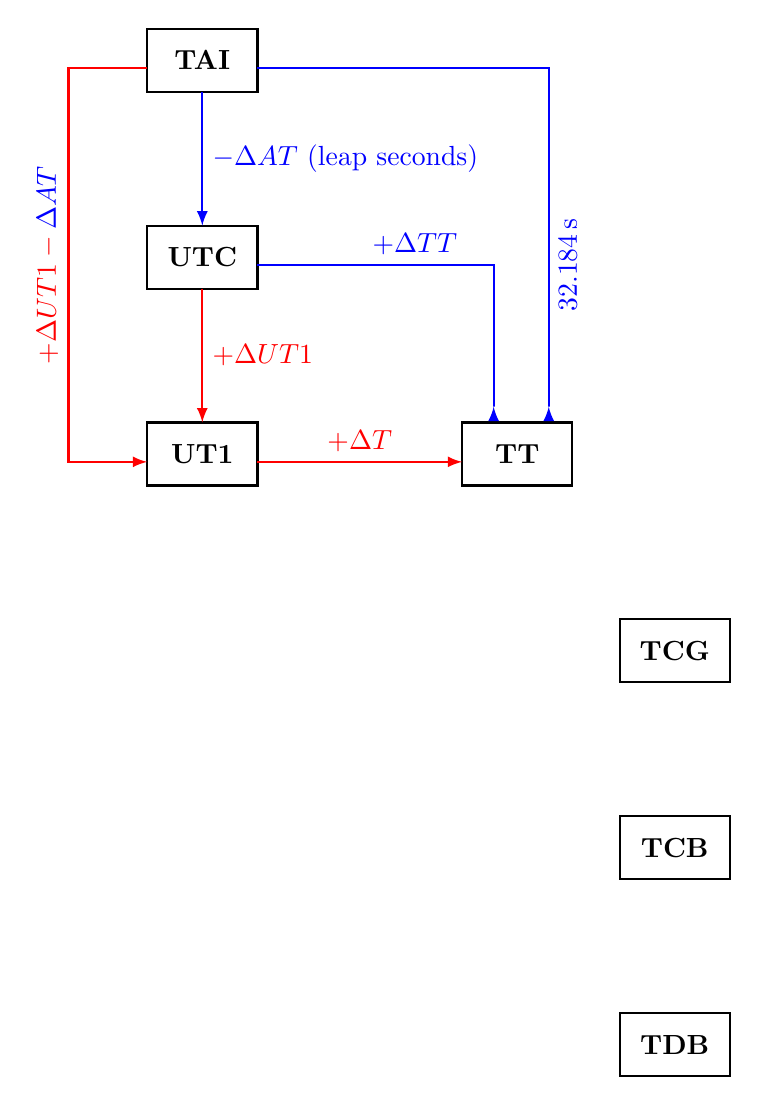
\begin{tikzpicture}
\coordinate (TAI) at (-4,5.0);
\coordinate (UTC) at (-4,2.5);
\coordinate (UT1) at (-4,0);
\coordinate (TT) at (0,0);
\coordinate (TCG) at (2,-2.5);
\coordinate (TCB) at (2,-5.0);
\coordinate (TDB) at (2,-7.5);

\draw [thick] (UT1) rectangle node{\textbf{UT1}}  ($(UT1)+(1.4,0.8)$);
\draw [thick] (UTC) rectangle node{\textbf{UTC}}  ($(UTC)+(1.4,0.8)$);
\draw [thick] (TAI) rectangle node{\textbf{TAI}}  ($(TAI)+(1.4,0.8)$);
\draw [thick] (TT)  rectangle node{\textbf{TT}}   ($(TT)+(1.4,0.8)$);
\draw [thick] (TCG) rectangle node{\textbf{TCG}}  ($(TCG)+(1.4,0.8)$);
\draw [thick] (TCB) rectangle node{\textbf{TCB}}  ($(TCB)+(1.4,0.8)$);
\draw [thick] (TDB) rectangle node{\textbf{TDB}}  ($(TDB)+(1.4,0.8)$);

\draw [>=latex,blue,thick,->] ($(TAI) + (0.7,0.0)$) -- node[anchor=west]{\(-\Delta AT\) (leap seconds)} ($(UTC) + (0.7,+0.8)$);
\draw [>=latex,red,thick,->] ($(UTC) + (0.7,0.0)$) -- node[anchor=west]{\(+\Delta UT1\)} ($(UT1) + (0.7,+0.8)$);
\path [>=latex,->,draw,red,thick] ($(TAI) + (0.0,+0.3)$) -| ++(-1,-2.5) node[rotate=90,above]{\(+\textcolor{red}{\Delta UT1} - \textcolor{blue}{\Delta AT} \)} |- ($(UT1)+(0.0,+0.3)$);
\path [>=latex,->,draw,blue,thick] ($(TAI) + (1.4,+0.3)$) -| ++(4.0-1.4+1.1,-2.5) node[rotate=90,below]{\( \SI{32.184}{\second} \)} |- ($(TT)+(1.1,+1.0)$);
\path [>=latex,->,draw,blue,thick] ($(UTC) + (1.4,+0.3)$) -| ++(3.0-1.4+0.4,0.0) node[rotate=00,above]{\( + \Delta TT \)} -| ++(1.0,0.0)node[]{} |- ($(TT)+(0.4,+1.0)$);
\draw [>=latex,red,thick,->] ($(UT1) + (1.4,0.3)$) -- node[above]{\(+\Delta T\)} ($(TT) + (0.0,+0.3)$);

\end{tikzpicture}
\caption{Timescale transformations, \cite{sofa_18161_tscb}}
\label{fig:time-scale-transformations}
\end{figure}

\subsection{Leap Seconds and $\Delta$AT}
\label{ssec:leap-seconds-dat}
Leap seconds are introduced when necessary to keep the time difference UT1-UTC 
to within \(\SI{\pm 0.9}{\second}\). They are injected at the end of December or 
June. Each time a leap second is introduced, the offset \(\Delta AT = TAI - UTC\) 
changes by exactly \SI{1}{\second} (leap seconds are in practice always positive, hence 
the offset is augmented, but provision for negative seconds exists if needed). In 
practice, are indicators of the accumulated difference between atomic time and time 
measured by Earth rotation. At the time of writing, the average solar day 
is now \SIrange{1}{2}{\milli\second} longer than the nominal \SI{86400}{\second}, accumulating 
to \SI{1}{\second} over a period of 18 months to a few years. As the Earth rotation 
slows, leap seconds will become ever more frequent.

The procedure of leap second injection, can be thought of as stopping the UTC clock 
for a second to let the Earth catch up.

\subsubsection{Leap Seconds Implications}
If a UTC date is not expressed using the hours, minutes, seconds format, but instead 
is expressed as a Julian Date (or MJD), an ambiguity will 
arise at the time of leap second injection. E.g., \cite{sofa_18161_tscb}, the dates 
June 30 1994, 235960.0 and July 1 1994, 000000.0 would both result to the same 
MJD, namely 49534.000; obviously, subtracting the two, identical JDs, would not 
yield the correct interval.

\subsection{Solar Time: UT1, UTC and $\Delta$UT1}
UT1 is the modern equivalent to \emph{mean solar time} and is really an angle rather 
than time (\cite{sofa_18161_tscb}). Historicaly its definition has involved the 
`ficticious mean Sun' and sidereal time, but now is defined through its relationship 
with Earth rotation angle. Because the Earth's rotation rate is slightly irregular
and is gradually decreasing, the UT1 second is not precisely matched to the SI second.
This makes UT1 itself unsuitable for use as a time scale in physics applications.
Nevertheless, it is still in use in a wide variety of applications.

Coordinated Universal Time (UTC) is the standard atomic based time scale in normal 
everyday use throughout the world. UTC is a compromise between the demands of 
precise timekeeping and the desire to maintain the current relationship between 
civil time and daylight (\cite{sofa_18161_tscb}).

To obtain UT1 starting from UTC, it is necessary to look up the value of 
\( \Delta UT1 = UT1 - UTC \) for the date concerned in tables published by the 
\gls{iers}; this is then added to the UTC. The quantity \(\Delta UT1\), which 
typically changes by \SIrange{1}{2}{\milli\second} per day, can be obtained only 
by observation, principally \gls{vlbi} using extragalactic radio sources, though seasonal effects 
are present and the \gls{iers} listings are able to predict some way into the future 
with adequate accuracy for most applications.

\( \Delta UT1 = UT1 - UTC \) is used to determine the \gls{era}, which is the 
angle measured along the intermediate equator of the \gls{cip} between the \gls{tio} and the 
\gls{cio} positively in the retrograde direction (\cite{IersBulABC04}; for details on 
\gls{era} computation, see \cite{iers2010}).

Values for \( \Delta UT1 \) are published by the \gls{iers} within the regularly disseminated 
\href{https://www.iers.org/IERS/EN/Publications/Bulletins/bulletins.html}{Bulletins}; 
\href{https://datacenter.iers.org/productMetadata.php?id=6}{Bulletin A} contains 
rapid determinations for earth orientation parameters, 
\href{https://datacenter.iers.org/productMetadata.php?id=207}{Bulletin B} 
contains monthly earth orientation parameters and 
\href{https://datacenter.iers.org/productMetadata.php?id=17}{Bulletin D} contains 
announcements of the value of \( \Delta UT1 \).

\subsection{$\Delta$T}
The difference between UT1 and TT (formerly ET) is called $\Delta$T, and in the 
present era can be written out as (\cite{sofa_18161_tscb}):
\begin{equation}
  \Delta T = TT - UT1 = \SI{32.184}{\second} + \Delta AT - \Delta UT1
\end{equation}

\section{Summary of Useful Formulas}
\label{summary-of-useful-formulas}

\begin{gather*}
  UT1 = UTC + (UT1 - UTC) \\
  TAI = UTC + \Delta AT \\
  TT \equiv TDT \approx ET \approx TAI + \SI{32.184}{\second} \\
  \Delta T = TT -UT1 = \SI{32.184}{\second} + \Delta AT - (UT1 - UTC)
\end{gather*}

\chapter{Technicalities}
\label{ch:technicalities}

\section{Software}
\label{se:software}

\begin{figure}
\centering
\begin{tikzpicture}[thick,scale=0.6, every node/.style={transform shape}]
  \path[mindmap,concept color=black,text=white]
    node[concept] {My Software}
    [clockwise from=0]
    child[concept color=green!50] {
      node[concept] {ggdatetime}
      %[clockwise from=90]
      %child { node[concept] {algorithms} }
    }
    child[concept color=blue!50] {
      node[concept] {sp3}
      %[clockwise from=-30]
      %child { node[concept] {databases} }
    }
    child[concept color=red!50]    { node[concept] {ggeodesy} }
    child[concept color=orange!50] { node[concept] {iers2010} }
    child[concept color=purple!50] { node[concept] {sinex} };
\end{tikzpicture}

\caption{Software Structure Tree}
\label{fig:software-structure-tree}
\end{figure}

\section{Dependencies}
\begin{description}
    \item [libcurl] a free, and open-source multiprotocol file transfer library.
    \href{https://curl.se/libcurl/}{libcurl} is highly portable, it builds and works 
    identically on numerous platforms and provides a \href{https://curl.se/libcurl/c/}{C API}, 
    accessing remote files via the C/C++ programming languages. Installation is 
    trivial in most operating systems\footnote{E.g. for Fedora LInux: \lstinline[language=bash]|$ dnf install libcurl libcurl-devel|}.
    
    \item [Eigen] (\cite{eigenweb}) a free, and open-source C++ template library 
    for linear algebra. 
    \href{https://eigen.tuxfamily.org/index.php?title=Main_Page}{Eigen} is a 
    versatile, fast and reliable library, with no dependencies other than the 
    C++ standard library. Since it is a header-only library, ``installation'' 
    and inclusion is very easy for any platform.

    \item [cgem] a free, and open-source C++ library. 
    \href{https://www.kthohr.com/gcem.html}{cgem} offers compile-time 
    computation of a number of widely used mathematical function, see
    \ref{sec:constexpr-math}

\end{description}

\section{Constexpr Math}
\label{sec:constexpr-math}
Currently (\today), the standard C++ library \texttt{math.h} does not offar 
trigonometric mathematical functions qualified as \texttt{constexpr} (see 
\href{https://en.cppreference.com/w/cpp/header/cmath}{Standard library header \texttt{<cmath>}}).
\texttt{constexpr} functions can spped-up computations by performing them at 
compile-time (see 
\href{https://en.cppreference.com/w/cpp/language/constexpr}{\texttt{constexpr} keyword}). 
The \href{https://gcc.gnu.org/onlinedocs/libstdc++/}{GNU C++ Library} 
implementation \texttt{libstdc++} does offer such functions as an extension. It 
was however decided to not use these extensions, because:
\begin{itemize}
    \item they do not conform to the standard,
    \item we want to be able to build with any compiler and standard library implementation
\end{itemize}

Hence, we are using the \href{https://www.kthohr.com/gcem.html}{Generalized Constant Expression Math} 
(\texttt{gsem}) library, when such functionality is needed.

It is expected that in the near future, most of the standard mathematical 
functions will be marked/implemented as \texttt{constexpr} (\cite{rostencpp}). 
When such functionality is offered, the dependency on \texttt{gcem} should be 
dropped in favor of using the standard functions.

Source files affected:
\begin{itemize}
    \item \path{occultation.cpp}
    \item \path{sunpos.cpp}
\end{itemize}


\bibliography{doris}

\glsaddall
\printglossary[type=\acronymtype,title=Acronyms]

\printindex

\end{document}
